\chapter{Theory}

%What to call this?
\section{General Rf theory}
To fully understand the theory of radio communications, it is important to have the fundamental understanding of parameters used to describe and measure the performance of a radio system. The next subsections will clarify the relation between gain and losses, power levels and also a description of how to use these parameters.

\subsection{Gain and loss}
The figure 2.1 below show an example of an electrical circuit. When a signal is generated and passes the circuit it can be amplified, attenuated or in an ideal world no change will happen to the signal. The strength of the signal can be measured at different points A,B or C and earth. 

\begin{figure}[h]
\centering
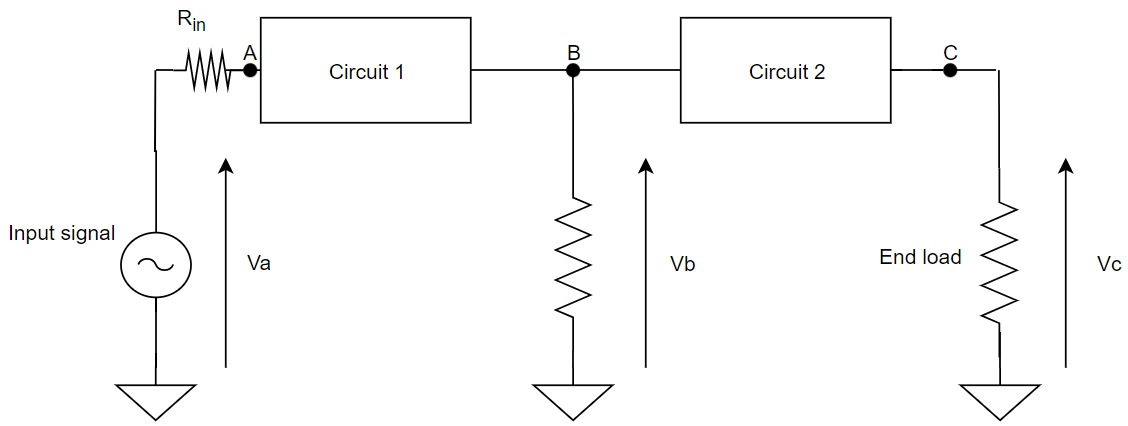
\includegraphics[scale=0.5]{figures/GainLoss.PNG}
\caption{Gain and loss}
\end{figure}

If the voltage level at B is greater than A then circuit 1 has provided an amplification to the original signal, a \textbf{Gain}. This gain is measured at the output of the whole circuit compared to the level at the input of the circuit.

$$GAIN_1 = \frac{V_B}{V_A}$$

If B is 10 Volts and A is 5 volts then circuit 1 will provide a Gain factor of 2 to the original signal, on the other hand if C was measured to be less than B, then circuit 2 will introduce a loss factor of 2:

$$LOSS_2 = \frac{V_B}{V_C} = \frac{10}{5} = 2$$

A general rule is to describe levels as \textbf{Gains} and not losses, such that the example above will be a gain factor of ½.

$$GAIN_2 = \frac{V_C}{V_B} = \frac{5}{10} = \frac{1}{2}$$

These principals applies to all radio communication system, the same goes for figure 2.2. The gain measure can be applied between any two points in a communication system, for example, the gain between the transmitter and receiver, in figure 2.2 is:

$$GAIN = \frac{V_B}{V_A}$$

\begin{figure}[h]
\centering
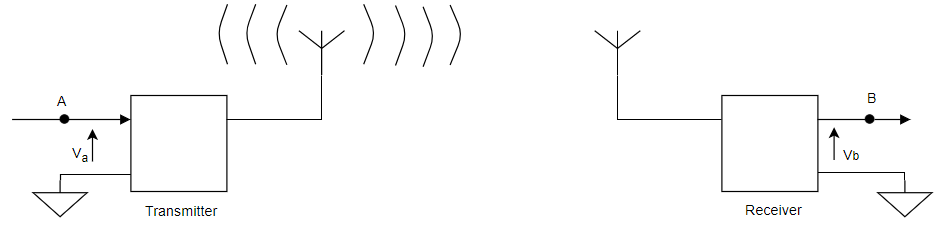
\includegraphics[scale=0.55]{figures/RadioCom.PNG}
\caption{Gain for a complete radio link system}
\end{figure}

\subsection{Power level}

Most radio systems measurements are made as measurement of power level, as seen below the equations for power are:

\begin{equation}
    P = V \cdot I
\end{equation}
\begin{equation}
    P = \frac{V^2}{R}
\end{equation}
\begin{equation}
    P = I^2 \cdot R
\end{equation}

where:\\

P = power (in watts)\\
V = voltage (in volts)\\
I = current (in amperes)\\
R = Load resistance (in ohm)\\

Alexander Graham Bell invented a unit of measure for sound levels. The unit is known as \textbf{Bel}, where one tenth of a bel is called a \textbf{decibel}. This is based on the human ear which hears in a logarithmic manner, thus a level of 100 watts to the human ear would sound twice as loud as a level of 10 watts, and not 10 times. This unit of measure is now used as the foundation for measuring relative power levels in the fields of electronics, acoustics, optics and many others. For figure 2.2, the gain of the radio system becomes: 

\begin{equation}
    GAIN = log_{10}\Big(\frac{P_B}{P_A}\Big)bels = 10 \cdot log_{10}\Big(\frac{P_B}{P_A}\Big)decibels
\end{equation}

The unit dB always expresses the logarithmic measurement of a power ratio, thus it has a meaning only if a reference level is set. That is why the above equation is for a relative measurement, which is a measure of the power level at point B with reference to the power level at point A - B relative to A. For example if the input signal at point A is 10 watts and 100 watts at point B, then the system gain is: written as 10dB. 

$$GAIN = 10 \cdot Log_{10}\Big(\frac{100}{10}\Big)$$
$$= 10 \cdot 1$$
$$= 10dB$$

For radio communication system, measurements can be made at a single points in a system with reference to 1 watt or 1 milliwatt (measurement of absolute power), thus the equations then becomes:

\begin{equation}
    LEVEL_{dBm} = 10 \cdot log_{10}\Big(\frac{P}{1W}\Big)
\end{equation}

\begin{equation}
    LEVEL_{dBW} = 10 \cdot log_{10}\Big(\frac{P}{1mW}\Big) = LEVEL_{dBm}-30dB
\end{equation}

\subsection{What is dB/dBi/dBd/dBW/dBm?}
Since this thesis is targeted towards the next generation of students in DanSTAR, it is worth explaining what the differences are between dB, dBi, dBd, dBW and dBm, to be crystal clear about the units. 

As explained in the section above dB is a logarithmic ratio of powers in reference to a given level. So saying $P_1 = 2 \cdot P_2$ is equivalent, to $\frac{P_1}{P_2}\overset{\Delta}{=} 3 dB$, because: 

\begin{equation}
    10 \cdot log_{10}\Big(\frac{P_1}{P_2}\Big)dB = 10 \cdot log_{10}(2)dB = 3dB
\end{equation}

dBi measures the gain over an isotropic antenna whereas dBd measures the gain over a half-wavelength dipole antenna, in section 2.5.1 \textit{Isotropic antenna)} and section 2.5.2 \textit{Directivity, efficiency and gain}, both units are explained in more details. What is important for now, is that a half-wavelength dipole antenna is estimated to have a gain of 2.15dBi, thus a 7.85 dBd means that the peak gain is 7.85 higher than a dipole antenna and 10 dB higher than a isotropic antenna, see figure 2.3 and the equation below:

\begin{equation}
    G(dBd) = G(dBi) - 2.15
\end{equation}

\begin{figure}[h]
\centering
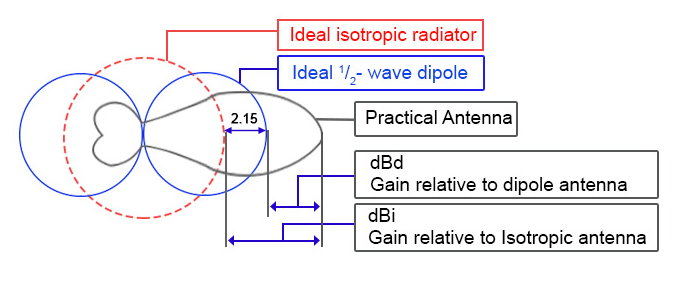
\includegraphics[scale=0.8]{figures/DBIvsDBD.PNG}
\caption{dBi vs dBd \cite{EverythingRF}}
\end{figure}

Both units dBi and dBd can be treated just like dB, because both, in the end, measures the again of an antenna relative to an isotropic antenna where the directivity is 1, resulting in a gain of 0dB.  

dBm and dBW is a logarithmic unit to measure powers. Since dB is a ratio of powers, dBm and dBW are both defined by forming the ratio of the power, relative to a reference power, which is 1W for dBW and 1mW for dBm, as formally explained in equation 2.5 and 2.6.  

\subsection{How (not) to use dB/dBi/dBd/dBW/dBm in relation to each other}
For clarity, this section is quite important for section 2.3 \textit{Link budget}, since the majority of the units are being used in the link budget.

Consequently, two thing are okay: 

Starting with a \textbf{power} (dBW and dBm) one can \textit{add} and \textit{subtract} ratios (db, dBi and dBd) as often as one desires with the end result of still having a power unit (dBW or dBm), although dBd needs to be converted to dBi unit, as shown in equation 2.8: 

\begin{equation}
\begin{split}
    P_1 \cdot \frac{G_1}{L_1} = P_2 \Leftrightarrow 10 \cdot log_{10}\Big(P_1 \cdot \frac{\frac{G_1}{L_1}}{1W}\Big) = 10 \cdot log_{10} \frac{P_2}{1W}\\
    \Leftrightarrow P_1|_{dBW} + G_1|_{dB} - L_1|_{dB} = P_2|_{dBW}
\end{split}
\end{equation}

Subtracting \textbf{two powers} (dBW or dBm) which is equivalent to computing their \textbf{ratio} (dB):

\begin{equation}
\begin{split}
    \frac{P_1}{P_2} \overset{\Delta}{=} 10 \cdot log_{10}\Big(\frac{P_1}{P_2}\Big) dB = 10 \cdot log_{10}\Big(\frac{P_1}{1W}\Big) - 10 \cdot log_{10}\Big(\frac{P_2}{1W}\Big) = P_1|_{dBW} - P_2|_{dBW}\\
    = 10 \cdot log_{10}\Big(\frac{P_1}{1mW}\Big) - 10 \cdot log_{10}\Big(\frac{P_2}{1mW}\Big) = P_1|_{dBm} - P_2|_{dBm}
\end{split}
\end{equation}

Both powers has to have the same unit, one can not mix between dBW and dBm. 

The above equations can be abbreviated to a simple "okay-to-do" table:

\begin{table}[h!]
\centering
\begin{tabular}{|c|}
\hline
$dBW  \pm dBi = dBW$\\
\hline
$dBm \pm  dBi = dBm$ \\ 
\hline
$dBW  \pm  dB = dBW$ \\ 
\hline
$dBm \pm dB = dBm$ \\  
\hline
$dBW - dBW = dB$ \\
\hline
$dBm - dBm = dB$ \\
\hline
\end{tabular}
\caption{What is allowed to do with the units dB/dBW/dBm/dBi}
\label{table:1}
\end{table}

Consequentially, three things are not okay to do:

One can never ever multiply dBW with dB. Example, an output power from a transceiver is $P_T = 10W$ with an antenna gain of $G_T = 10$ gives an effective radiated power of 100 dBW, this is not true since 100 dBW is practically 10 Gigawatts! Multiplication in linear scale becomes addition in logarithmic scale: 

\begin{equation}
\begin{split}
    P_T \cdot G_T = 10W \cdot 10 = 100W \overset{\Delta}{=} 20dBW\\
    \Leftrightarrow  P_T|_{dBW} + G_T|_{dBi} = 10dBW + 10dBi = 20dBW  
\end{split}
\end{equation}

For equation 2.11 see also table 2.1 first row. 

Furthermore, one can not add a bunch of power quantities in dBW or dBm! Adding powers in log scale means multiplying them in linear scale, for example:  

\begin{equation}
    10dBW + 3dBW + 6dBW \overset{\Delta}{=} 10W \cdot 2W \cdot 4W = 80W^3
\end{equation}

The above equation 2.12 does not make sense, since one can wonder what Watt cubed even means?

Lastly, by now one can already deduce that power can not be measured in dB and gain/loss can not be measured in dBm or dBW. 

\section{A general radio communication system}
The general overview of any point-to-point radio communication system, is always the same. There is a sender (Tx) and a receiver (Rx), now a days the sender and receiver is build into one system, called a transceiver. Some transceivers has internal Power Amplifiers (PA) and internal Low Noise Amplifiers (LNA). The internal PA amplifies the signal when the transceiver is in transmitting mode, and the LNA filters the signal when the transceiver is in the receiving mode.

On figure 2.4, both the transmitter and the receiver has an antenna. When the transmitter starts to transmit, an analog radio wave is generated from the transmitter that travels to the antenna to be amplified (in correct terms the antenna directs the radio wave), and then it propagates out through space. When the radio wave travels through space, it will encounter different phenomenons, which will introduce losses to the system. Once the radio wave has reached the receiver it will be detected by its antenna, thus the signal will travel to the chip and gets turned to a digital signal.

\begin{figure}[h]
\centering
%\hspace{-1cm}
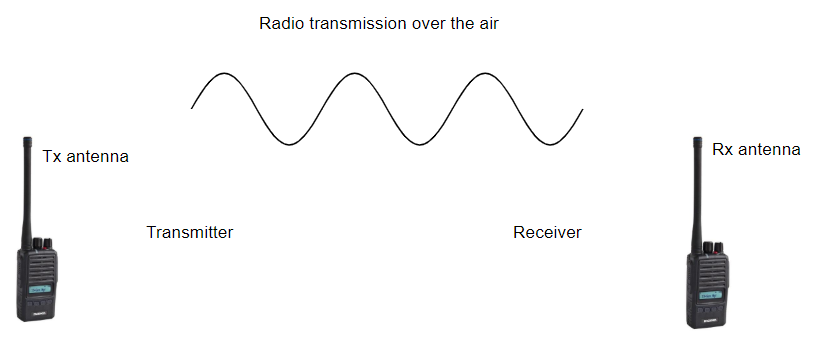
\includegraphics[scale=0.55]{figures/GeneralOverview.PNG}
\caption{General overview of a point-to-point radio communication system}
\end{figure}

\subsection{RF propagation}
Radio signals can travel over vast distances. However they are affected by the medium in which they travel through. Depending on which frequency band is used\cite{FrequencyBand}, some can propagate around the globe, whereas other radio signals may only travel over much shorter distances.

There are many different factors that affect the way in which radio signals travels through a medium - since this thesis is about a radio communication system for a rocket that flies through the air, it is only the free-space propagation (atmosphere) medium that is considered. These factors can be various objects that may appear in the path. Furthermore, The radio wave may be subjected to reflection, refraction and diffraction. The received radio signal may also be a combination of several signal that have traveled by multiple paths, these multi-path signals will interfere with each other and cause constructive and destructive interference, meaning the signal might get stronger or weaker. Because the signals are propagating through different paths, some may be delayed causing the received signal to be distorted. It is therefore important to understand these factors, in order to get an idea about which one has the biggest affect on the radio signal. 

There are a number of media in which RF propagates through, these are: 

\begin{itemize}
  \item \textbf{Free-space Propagation:} Also called Line-of-sight propagation (LOS). Here the radio signals will travel in free space, or away from any objects that may influence the propagation of the signal. Thus, it is only the distance from the source that affects the signal strength. This type of radio signal is seen with ordinary radio communication systems: HAM radio, cellular communication, satellites etc. As stated above, this medium the biggest factor in which this thesis is based on. 
  \item \textbf{Ground wave propagation:} The signal travels above the ground and is modified by the type of ground or terrain over which it travel. For low frequency bands the radio wave tends to follow Earth's curvature, this allows for long range communication below horizon.  
  \item \textbf{Ionospheric propagation:} Here the radio wave is reflected by the ionosphere (a region in the atmosphere where the air molecules have been ionized by the sun to allow for free electrons, starts around 60km) back to earth surface. The radio wave is reflected multiple times, causing a scattering of the original signal back to earth. This form of propagation can allow for short wave bands to reach the other side of the globe.
  \item \textbf{Tropospheric propagation:} The radio wave is reflected by the troposphere (effects starts around 2km), due to higher air density and higher water vapour at lower altitudes, this results in higher refractive index compared to higher altitude, which in the end reflects the radio wave. Like the ionospheric propagation, the tropospheric propagation also result in a scattered pattern of the incoming radio wave. 
\end{itemize}

%%FOR more details read this book IDC technology etc..

\subsection{Radio frequency bands}
The radio spectrum extends from 3Hz to 3THz. In between this spectrum sub-band has been defined by the International Telecommunication Union (ITU)\cite{ITU}. Figure 2.5 depicts the radio spectrum in defined bands. In this thesis the Industrial, scientific and medical radio bands (ISM)\cite{ISM} is used, specifically the 2.4-2.5Ghz spectrum, since this spectrum is mostly open worldwide, allowing us to design one system that can be used both in USA and in Europe without any change to the hardware.   
\begin{figure}[h]
\centering
%\hspace{-1cm}
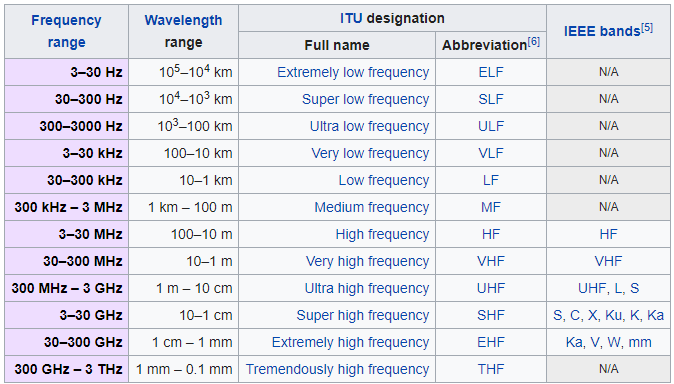
\includegraphics[scale=0.8]{figures/radioSpectrum.PNG}
\caption{Radio spectrum and sub-bands\cite{FrequencyBand}}
\end{figure}

\section{Radio channel losses and other losses}
It is important for a communication system to be designed for the intended environment and to predict with relative certainty, the performance of the system prior to fabrication and implementation. Insufficient planning can result in over-design and wanted resources or under-design and poor performance. Before planning the communication system, it is important to understand the essential parameters of each sub-link. Some of these parameters are given or chosen during the design process, while others has to be calculated, these include: Free-space attenuation, Multipath attenuation, Fresnel zone, Atmospheric attenuation, Rain attenuation, cloud attenuation and others. Figure 2.6 showcases some of these phenomenons, especially free-space and multipath attenuation. 

\begin{figure}[h]
\centering
%\hspace{-1cm}
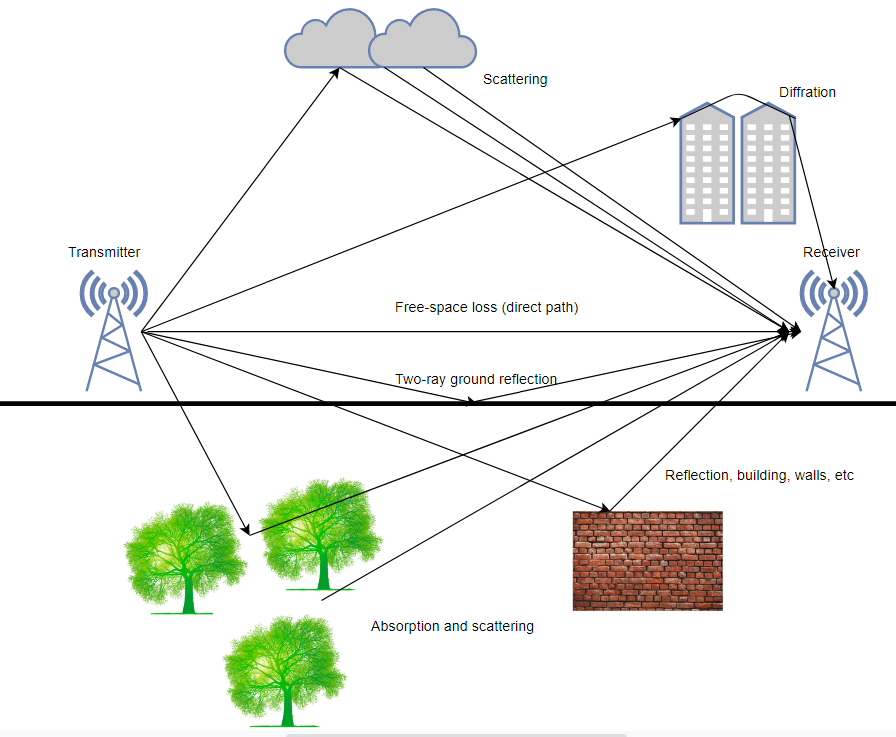
\includegraphics[scale=0.6]{figures/Multipath.PNG}
\caption{Radio wave can propagate through multiple paths}
\end{figure}

Before looking into the theory of the detailed link budget, the theory of the above parameters will be clarified in the following sections.

%Maybe Before looking into the theory of the antennas, the theory of the above parameters will be clarified in the following sections.

\subsection{Free-space attenuation}
When a radio wave propagated through space it will start to disperse in a spherical form, this dispersion or "spread out" of the radio beam will result in a loss. This loss is consistent and is tight to the wavelength, which means that it increases with frequency as the wavelength becomes shorter. This phenomenon is called free-space loss and is related to both the frequency and the slant range (direct path), which is the distance between the transmitter and receiver antenna. The free-space loss is derived by Friss transmission equation: 

\begin{equation}
    \frac{P_{Rx}}{P_{Tx}} = G_T \cdot G_R \Big( \frac{\lambda}{4 \cdot \pi \cdot d} \Big)^2
\end{equation}

Where:

\begin{itemize}
  \item $P_{Rx}$ is the power fed into the transmitting antenna input terminals.
  \item $P_{Tx}$ is the power available at receiving antenna output terminals.
  \item $G_T$ is the gain of the transmitting antenna.
  \item $G_R$ is the gain of the Receiving antenna.
  \item $d$ is the distance between the transceivers in meters.
  \item $\lambda$ is the wavelength.
\end{itemize}

To derive the Path loss equation, it is assumed that the antennas are isotropic, which means they both have a gain of 1, resulting in:

\begin{equation}
    \frac{P_{Rx}}{P_{Tx}}|_{iso} =  \frac{\lambda^2}{4^2 \cdot \pi^2 \cdot d^2}
\end{equation}

% The path loss is a dB ratio of $\frac{P_{Tx}}{P_{Rx}}$, which gives: 

% \begin{equation}
%     \frac{P_{Tx}}{P_{Rx}}|_{iso} =  \frac{4^2 \cdot \pi^2 \cdot d^2}{\lambda^2}
% \end{equation}

Converting to dB:

\begin{equation}
    L_{fs,dB} =  10 \cdot log_{10}\Big(\frac{\lambda^2}{4^2 \cdot \pi^2 \cdot d^2}\Big) \Leftrightarrow 10 \cdot log_{10}\Big(\frac{\lambda}{4 \cdot \pi \cdot d}\Big)^2 \Leftrightarrow 20 \cdot log_{10}\Big(\frac{\lambda}{4 \cdot \pi \cdot d}\Big) 
\end{equation}

Since, $\lambda = \frac{f}{c}$, where f is the frequency and c is the speed of light (m/s), it is possible to substitute this in the final equation:

\begin{equation}
    L_{fs,dB} = 20 \cdot log_{10}\Big(\frac{c}{4 \cdot \pi \cdot d \cdot f}\Big) 
\end{equation}

What can be deduced from equation 2.16 is that doubling the output power from a transmitter does not equal to a doubling of the distance, in fact one has to quadruple the power before doubling of the distance occurs. A simple example is shown below:

Assume $\lambda = 1$ and $L_{fs,dB} = 0$

\begin{equation}
    0 = 20 \cdot log_{10}\Big(\frac{1}{4 \cdot \pi \cdot d}\Big)
\end{equation}

solving for d:

\begin{equation}
    d = 1/(4*Pi) = 0.079578
\end{equation}

To reach double the distance, one has to multiply d by 2 and substitute it in equation 2.17:

\begin{equation}
   L_{fs,dB} = 20 \cdot log_{10}\Big(\frac{1}{4 \cdot \pi \cdot 2 \cdot 0.079578}\Big) = 6.02dB 
\end{equation}

From 0dB to 3dB is in linear form a doubling factor, whereas from 0dB to 6dB, as seen in equation 2.20, is in linear form a quadrupling factor.

%% Write that in the section "calculation" we will go through this more in detail

\subsubsection{Received signal level}
Received signal level (RSL), is the power (measured in dbm) received at the receiver end. RSL can be deduced from Friss transmission equation, by simply solving for $P_{Rx}$, which yields the formula:

\begin{equation}
    P_{Rx} = P_{Tx} \cdot G_T \cdot G_R \Big( \frac{\lambda}{4 \cdot \pi \cdot d} \Big)^2
\end{equation}

The above equation can be used to figure out how good the received signal is, but also use the RSL to track object. This can be done by pointing the receiver antenna towards the transmitter antenna, and if any RSSI is observed then one can confirm that the antennas are pointing towards each other. It is important to know that with this method mulitpath signals and other phenomenons are not excluded, which is why this method require a clear LOS path between the transmitter and receiver. Furthermore, the above equation does not include losses from PCB design or components, like band filters, balun and Low-noise amplifiers (LNA). The receives signal strength identification (RSSI) will include the losses of the components, since this value is read from the transceiver, which is placed after the losses of band filter and baluns.    

\subsection{Multipath attenuation}
The above section 2.5.1 \textit{free-space attenuation} applies to the fact that the radio wave
propagating in a direct path from the source to the receiver. This section, looks behind the theory of multipath, where the radio wave is propagating differently from the desired, or direct path. The amplitude, phase and angle-of-arrival of the multipath signal interfere with the amplitude, phase and angle-of-arrival for the direct signal. This interference can create error in the phase, amplitude or angle-of-arrival. As explained in section 2.3 \textit{RF propagation}. The amplitude can be larger of smaller depending on whether the multipath signal creates a constructive or destructive interference, see then next section. The problem with multipath is that the source signal travels in multiple paths, as seen on figure 2.6 and ends up interfering with itself at the receiving end. The reflected path has a reflection coefficient that determine the phase and the amplitude of the reflected signal, which is not the same as the direct path. Since the reflected path is longer than the direct path, it will produce a signal with a different amplitude phase at the receiving end. For example if the reflected signal is 180 out of phase from the direct path and the amplitude are the same, then the signal is canceled out which makes the receiver detecting little to no signal. Luckily, since the reflected signal takes a longer path it will also experience more free-space attenuation, which makes the amplitude of the reflected signal lower than the direct path, thus reducing the attenuation of the signal that is out of phase compared to the direct path. Figure 2.6 shows, that there are multiple parameters at play for calculating the total loss of a signal traveling towards the receiver. Therefore, it is generally hard to quantify the loss due to multipath. Since the rocket is constantly moving, multipath will constantly be changing, which in return will result in a variable channel loss. 

The following next sub-sections will explain the key parameters that affects the rocket, but also when range test on the ground is conducted. 

\subsubsection{Two-ray ground bounce multipath}
The theory and formulas of this section is derived from what is written in the book \textit{Introduction to RF Propagation - John s. Seybold}\cite{RFpropagation} from page 164 to 173, it is highly recommended to read these pages. Wikipedia also has an article\cite{Two-ray} about how the two-ray ground bounce works, although the formula is derived differently but with the same final equation as from the book. 

%%there many ground bounce multipath model 3-ray 4-ray 10-ray etc. 

Since testing the radio communication system will be done on the ground, it is important to factor in near-earth propagation path. There are two key effects: ground reflection and path blockage and/or diffraction when part of the path is beyond line of sight. When the radio wave propagates near the earth's surface and parallel to it, severe fading can occur if the ground is reflective. 

Below on figure 2.7 the two-ray ground bounce model can be observed. Consider a point-to-point radio link system that is operating close to earth's surface. For this example it is assumed that the ground is flat, smooth and reflective. This means that there is a "specular" ground reflection\cite{specular} from the ground plane. Specular reflection occurs if and only if the angle of the incidence equals to the angle of the angle of the departure at the reflection point (or the normal plane), thus $ø_1 = ø_2$. 

\begin{figure}[h]
%\centering
\hspace{-0.5cm}
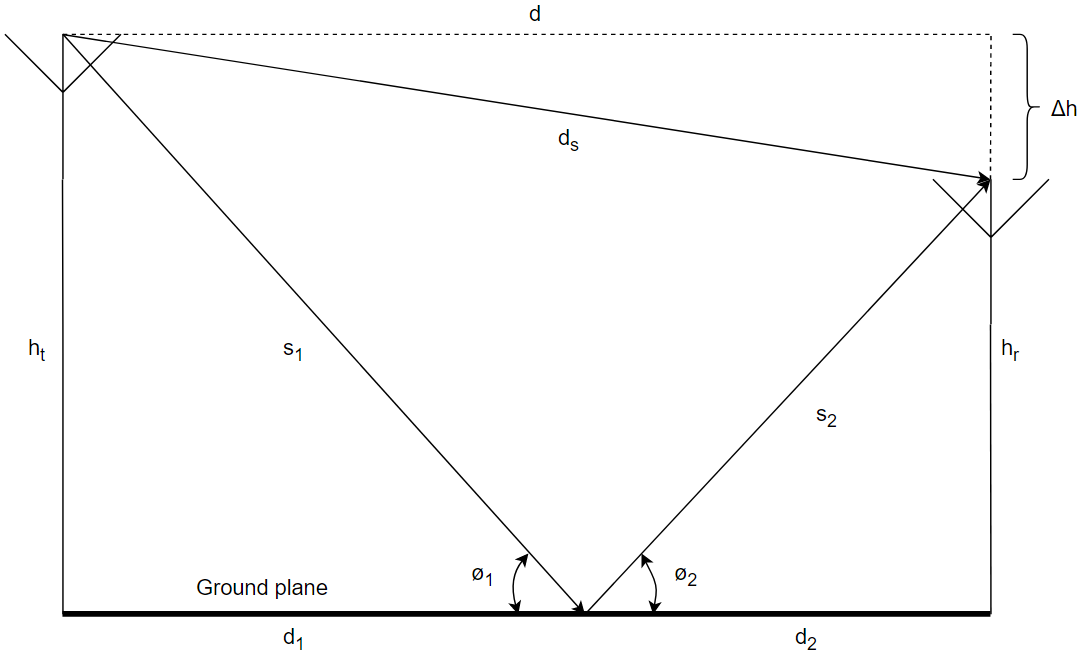
\includegraphics[scale=0.6]{figures/TwoRay.PNG}
\caption{Two-ray ground bounce model}
\end{figure}

On figure 2.7 it can be observed that:

$$ø_1 = ø_2$$

The slant range is:

\begin{equation}
  d_s = \sqrt{d^2 + (h_t - h_r)^2}= \sqrt{d^2 + \Delta h^2}
\end{equation}

and 

\begin{equation}
  d = d_1 + d_2
\end{equation}

The reflection angles are:

$$ø_1 = tan^{-1}\Big(\frac{h_t}{d_1}\Big), \quad ø_2 = tan^{-1}\Big(\frac{h_r}{d_2}\Big)$$

Since the two angles are equal to each other, it is clear that: 

$$\frac{h_t}{d_1} = \frac{h_r}{d_2}$$

Using (2.22) the above equation will be:

\begin{equation}
  d_1 \cdot h_r = (d-d_1) \cdot h_t
\end{equation}

solving for $d_1$ results in:

\begin{equation}
  d_1 = \frac{d \cdot h_t}{h_r + h_t}
\end{equation}

Replacing $d_1$ by $d - d_2$ in (2.23) and solving for $d_2$, results in the following equation:

\begin{equation}
  d_2 = \frac{d \cdot h_r}{h_r + h_t}
\end{equation}

Thus the specular reflection point between the two antennas can be calculated by knowing the heights of the antennas. From specular geometry the following equations can be derived: 

\begin{equation}
  s_1 = \sqrt{d_1^2 + h_t^2} = h_t \cdot \sqrt{1 + \frac{d^2}{(h_r + h_t)^2}}
\end{equation}

\begin{equation}
  s_2 = \sqrt{d_2^2 + h_r^2} = h_r \cdot \sqrt{1 + \frac{d^2}{(h_r + h_t)^2}}
\end{equation}

As described in the book \textit{Introduction to RF Propagation - John s. Seybold}\cite{RFpropagation} page 166. The magnitude and phase of the reflected signal $s_2$ are determined by the path-length difference and reflection coefficient of the ground plane. The reflected signal is changed by the reflection coefficient, denoted $\rho$, for both the magnitude and phase parameters. For a smooth, reflective surface, the magnitude of the reflection coefficient is approximately 1, regardless of the polarization and frequency, if grazing angle is mall. See the figures on page 167 to 168 in the book \textit{Introduction to RF Propagation - John s. Seybold}\cite{RFpropagation}. For vertical polarization the phase angle is 180-degrees. For horizontal polarization it is virtually 180-degrees, regardless of frequency and grazing angle. For our test setup the grazing angle is very small, thus the reflection undergoes a 180-degree phase shift at he point of reflection regardless of polarization, this means that $|\rho| = 1$.

For a setup where $d_s > h_t$ and $d_s > h_r$ meaning gazing angle $ø$ is very small, the following approximation can be made:

$$s_1 + s_2 \approx d_s$$

The above equation states that since the reflected path is equal to the direct path, then the waves are exactly in phase, meaning there will be a 6dB increase in the received signal, since doubling the amplitude means quadrupling the power. If the reflected wave is exactly 180-degree out of phase then the signal will cancel completely and no signal will be received.

Over a flat, reflective surface, the magnitude of \textbf{E} field at the receiver can be expressed as: 

\begin{equation}
  |\textbf{E}| = |E_d| \cdot 2 \cdot sin(\Delta\phi/2)
\end{equation}

where $\Delta\phi$ is the phase difference due to path-length difference and $E_d$ is the \textbf{E} field due to the direct return only. The phase difference $\Delta\phi$ between the direct and reflected wave is:

\begin{equation}
  \Delta\phi = \frac{s_1 +s_2 - d_s}{\lambda} \cdot 2 \cdot \pi
\end{equation}

Substituting (2.21), (2.26) and (2.27) into (2.29) yields:

\begin{equation}
  \Delta\phi = d\Bigg( \sqrt{1+ \frac{(h_r+h_t)^2}{d^2}} - \sqrt{1+ \frac{(h_t+h_r)^2}{d^2}} \Bigg) \frac{2\pi}{\lambda}
\end{equation}

$\Delta\phi$ can be derived by using binomial expansion for the square roots.

Binomial expansion is given by: 

$$\sqrt{1+x} = 1+\frac{x}{2}-\frac{x^2}{8}+\frac{x^3}{16}-\frac{x^4}{16}+..$$

In the binomial expansion, it can be observed that if $d>>h_r$ and $d>>h_t$, then:

$$x=\Big(\frac{h_r+h_t}{d}\Big)^2 \approx 0 , \quad x=\Big(\frac{h_r-h_t}{d}\Big)^2 \approx 0$$

Using only the first two terms of the binomial expansion, (2.30) be simplified to:

\begin{equation}
  \Delta\phi\cong \frac{2h_rh_t2\pi}{d\lambda}
\end{equation}

The received power is proportional to the magnitude squared of the \textbf{E} field:

$$P_{rx} \propto |\textbf{E}|^2$$


Therefore substituting (2.31) into (2.28) using the above equation, yields:

\begin{equation}
  P_{rx} = 4 \frac{|E_d|^2}{\eta}sin\Big(\frac{2 \pi h_th_r}{d\lambda}\Big)^2
\end{equation}

From the free-space loss equation (2.13), see section 2.5.1 \textit{Free-space attenuation}, the magnitude squared of the direct path \textbf{E} Field at the receiver, $E_d$, is given by:

\begin{equation}
  |E_d|^2 = \eta \frac{P_{tx}G_TG_R\lambda^2}{(4\pid)^2} \Rightarrow \frac{|E_d|^2}{\eta} = \frac{P_{tx}G_TG_R\lambda^2}{(4\pid)^2}
\end{equation}

where $\eta$ is the characteristic impedance of free space. So substituting (2.33) into (2.32) gives:

\begin{equation}
  P_{rx} = 4 \frac{P_{tx}G_TG_R\lambda^2}{(4\pi d)^2}sin\Big(\frac{2 \pi h_th_r}{d\lambda}\Big)^2
\end{equation}

Assuming $d>>h_t$, $d>>h_r$ and $d\lambda << h_th_t$, then the following approximation may be made:

$$sin\Big(\frac{2 \pi h_th_r}{d\lambda}\Big)^2=\Big(\frac{2 \pi h_th_r}{d\lambda}\Big)^2$$

Thus:

\begin{equation}
  P_{rx} = 4 \frac{P_{tx}G_TG_R\lambda^2}{(4\pi d)^2}\Big(\frac{2 \pi h_th_r}{d\lambda}\Big)^2
\end{equation}

Resulting in the following approximate expression for the path loss on a near-earth propagation path over a flat, smooth, reflecting surface:

\begin{equation}
  L_{mp}= G_TG_R \frac{(h_th_r)^2}{d^4}
\end{equation}

Converting (2.34) to dB by assuming the antennas are isotropic with a gain of one, yields:

\begin{equation}
\begin{split}
  L_{mp,dB}|_{iso} = 10 \cdot log_{10}\Big(\frac{h_t^2h_r^2}{d^4}\Big) \Rightarrow 20 \cdot log_{10}\Big(\frac{h_th_r}{d^2}\Big) \\ \Rightarrow  20 \cdot (log_{10}\Big(h_th_r\Big) - 2 \cdot log_{10}\Big(d\Big)\Big) \\ \Rightarrow  20 \cdot log_{10}\Big(h_th_r\Big) - 40 \cdot log_{10}\Big(d\Big)
\end{split}
\end{equation}

It is worth notifying that this two-ray ground bounce path loss expression (2.35) is independent of the wavelength compared to the standard path-loss formula (2.14). The recommended approach to figure out which one of the two (2.14) and (2.35) formula to use, is to compute both of them plot them in a graph and use whichever one gives the greater loss. 

A helpful tool is to determine the crossover point, which is defined as the distance at which the $1/d^4$ approximation and free-space loss are equal. This crossover point can be used to figure out which one of the above formulas should be used at what distances. The crossover point is found by equating the approximate ground bonce path loss (2.35) and free-space loss (2.14) and solving for d:

$$\frac{(h_th_r)^2}{d^4}=\Big(\frac{\lambda}{4 \pi d}\Big)^2$$

\begin{equation}
  d_x= \frac{4\pi h_th_r}{\lambda}
\end{equation}

\subsubsection{Fresnel Zone}
In any radio wave propagation between a transmitter and a receiver, some amount of the radiated wave propagates off-axis, due to the expansion of the wave in a spherical form. These waves can then deflect off of objects and then travel to the receiver. As explained in the above section 2.5.2.1 \textit{two-ray ground bounce} the direct-path wave and the deflected-path wave may arrive out-of-phase or in-phase causing either destructive or constructive interference. The fresnel zone are prolate ellipsoidal shaped regions in space (n=1,2,3...), see figure 2.8, centered around the line of direct transmission between the transmitter and receiver, path TR on figure 2.8 below. 

The 1st region $n=1$ includes the space in which the LOS signal passes through. If a radio signal of the transmitted signal bounces off an object (the object could be anything: house, car, humans etc) within this region and then arrives at receiving antenna, the phase shift will be less than a quater-length wave or less than 90-degrees, Path TPR. The effect of phase-shift \underline{alone} in this region is minimal, therefore it can potentially result in having a positive impact on the receiver end, as the signal interferes with itself (direct path and bounced path), causing an in-phase interference, where the sum of the amplitude doubles. However, the positive outcome of this deflection also depends on the polarization of the signal relative to he object. %see section about polarization, where is it???????!!!!!!  

The 2nd region $n=2$ surrounds the 1st region but excludes the first region. If an object is located in this region, the signal that bounces of this object towards the receiver, will be shifted more than 90-degrees, but less than 270-degrees, because of the increased path length. This bounced signal will potentially be received out-of-phase, though again it depends on the polarization of the signal.

The 3rd region $n=3$ surrounds the 2nd region and deflected the waves towards the receiver in the same manner as the 1st region, because the wave have shifted more than 270-degrees but less than 450-degrees (ideally 360-degree shift will cause the best interference), therefore the signal may arrive as the same shift as the 1st region. 

The 4th region is the same as the 2nd region, and so on. In fact the fesnel zone consists of infinite regions. The further out in regions the signal get bounced back the less of an effect it has on the receiver end, because of the increased path loss.\cite{FesnelZone}  

\begin{figure}[h]
%\centering
\hspace{-3cm}
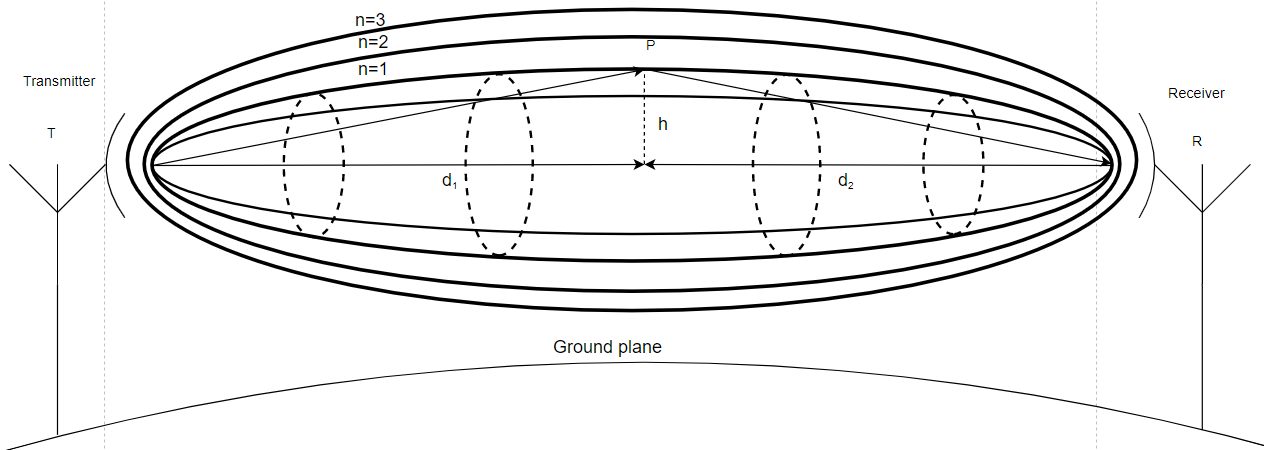
\includegraphics[scale=0.6]{figures/FresnelZoneN.PNG}
\caption{Fresnel zone model}
\end{figure}
The theory below is described in the book \textit{Introduction to RF Propagation - John s. Seybold}\cite{RFpropagation} page 175 to 178.
Consider a point-to-point radio system depicted on figure 2.8. The vector TR is the LOS path, between the transmitter and receiver, therefore the link distance it $d_1 + d_2$. The direct and reflected/diffracted path lengths can be expressed as: 

$$TR=d_1 + d_2$$

$$TPR=\sqrt{d_1^2+h^2}+\sqrt{d_2^2+h^2}$$

So the difference in path length is:

\begin{equation}
  TPR-TR = \Delta = \sqrt{d_1^2+h^2}+\sqrt{d_2^2+h^2}-d_1-d_2
\end{equation}

The binomial expansion can be used if $h<<d_1$ and $h<<d_2$:

$$\sqrt{d_1^2+h^2} \cong d_1 \Big(1+\frac{h^2}{2d_1^2} \Big) $$

and

$$\sqrt{d_2^2+h^2} \cong d_2 \Big(1+\frac{h^2}{2d_2^2} \Big) $$

Substituting it in (2.38), yields:

\begin{equation}
  \Delta=d_1+\frac{h^2}{2d_1}+d_2+\frac{h^2}{2d_2}-d_1-d_2 = \frac{h^2}{2d_1} + \frac{h^2}{2d_2} = \frac{h^2}{2}\Big(\frac{d_1+d_2}{d_1d_2}\Big)
\end{equation}

The corresponding phase difference is: 

$$\phi = \frac{2\pi \Delta}{\lambda}$$

Substituting (2.39) in the above equation, becomes: 

\begin{equation}
  \phi = \frac{2\pi}{\lambda} \cdot \frac{h^2}{2}\Big(\frac{d_1+d_2}{d_1d_2}\Big)
\end{equation}

The case where $\Delta = \frac{n\lambda}{2}$, where n is an integer, can found by letting  $\phi = n\pi$ in (2.40):

\begin{equation}
  n\lambda=h^2\Big(\frac{d_1+d_2}{d_1d_2}\Big)
\end{equation}

The destructive reflection/diffraction points can be identified by defining a term $h_n$, where n is the region in Fresnel zone and reorganizing the equation (2.41), which results in:

\begin{equation}
  n\lambda=h_n^2\Big(\frac{d_1+d_2}{d_1d_2}\Big)\Rightarrow h_n^2= \frac{n\lambda}{\frac{d_1+d_2}{d_1d_2}}=\frac{n\lambda d_1d_2}{d_1+d_2} => h_n = \sqrt{\frac{n\lambda d_1d_2}{d_1+d_2}}
\end{equation}

The final general equation for calculating the Fresnel zone radius at any point P between the endpoints of the LOS is the following formula: 

\begin{equation}
h_n = \sqrt{\frac{n\lambda d_1d_2}{d_1+d_2}}
\end{equation}

where:

\begin{itemize}
  \item $d_1,d_2>>n\lambda$ and $n \neq 0$
  \item $h_n$ is the nth Fresnel zone radius.
  \item $d_1$ is the distance of P from transmitter
  \item $d_2$ is the distance of P from transceiver
  \item $\lambda$ is the wavelength of the transmitted signal.
\end{itemize}

As explained in the beginning of this section the Fresnel zone can be used to determine if the received signal is in-phase or out-of-phase, but the polarization of the transmitted signal can greatly influence how the signal is received. The RF signal can be transmitted in different ways, described in section 2.8.1.5 \textit{Polarization}.

If a signal is vertically polarized and it deflects off a horizontal object, like a flat roof, and then bounces towards the receiving antenna, and if the roof is within the 1st region of the Fresnel zone, the resulting signal will be inverted relative to the original transmitted signal. Hence, even though one would expect a minimal change in phase in the 1st region, the bounced signal will arrive out-of-phase, due to the inverted signal, causing little to no signal at the receiving end. There are a multiple ways to solve this problem. One is to increase the height of the antennas such that the flat roof is in the 2nd Fresnel region, so that the inverted signal will be in-phase at the receiving end, read the beginning of this section about the 2nd Fresnel zone. Another way is to change the polarization of the antennas on both the transmitter and receiver side to to horizontal polarization, but staying in the 1st Fresnel zone. 

If the transmitted signal is circular polarized, then Fresnel zone does not matter, since a deflected circular polarized signal will change its rotational polarization, such that the received signal will be inverted to the receiving antenna, this will result in no signal received, whether is arrives in-phase or out-of-phase does not matter either. 

It is important to state that the Fresnel zone calculation does not return a specific dB loss which then can be used in the Link budget calculation, rather it is used as a rule of thumb having 60\% of the 1st region of the Fresnel zone to be clear is sufficient enough for a good radio link. The 60\% clearance applies to the radius of the ellipsoid, meaning $0.6h_n$ should be cleared. The next section will explain how the Fresnel-Kirchhoff diffraction parameter is used to give an estimate of the loss (in dB) in the Fresnel zone. 

\subsubsection{Single Knife-edge diffraction attenuation}
Diffraction is the physical phenomenon that occur when a wave encounters an obstacle. It is defined as the bending of waves around the corners of an obstacle, that obscure the line of sight. Diffraction has the effect of filling in shadows, so that some amount of electromagnetic energy will be present in the shadowed region. A short explanation to this phenomenon is in term of Heygen's Principle, which states that each point on a wavefront acts as the source of a secondary "wavelet" and all of these "wavelets" combine to produce a new wavefront in the direction of propagation.\cite{Huygens}. If an object is blocking part of the propagating wavefront, then the "wavelets" near the blockage will travel in direction other than that of the plane wave, which results in diffraction. Regardless of whether the blockage is conductive or not diffraction will still occur.

To accurately model the loss due to diffraction is very challenging for all but the most basic geometries. The easiest geometry to model the diffraction off is the \textit{knife-edge diffraction}, it can be used to provide an estimate of the diffraction loss for a single knife-edge blockage. The electrical field due to the diffracted path is given by the diffraction integral, which is approximated to be, see the book \textit{Mobile Communications Engineering: Theory and Applications} by Dr. William Lee, on page 142:

\begin{equation}
    L_r = 0 dB, \quad v \leq -1
\end{equation}

\begin{equation}
    L_r = 20log_{10}(0.5-0.62v) dB, \quad -1\leq v\leq0
\end{equation}

\begin{equation}
    L_r = 20log_{10}(0.5e^{-0.95v}) dB, \quad 0\leq v\leq 1
\end{equation}

\begin{equation}
    L_r = 20log_{10}(0.4-\sqrt{0.1184-(0.38-01v)^2}) dB, \quad 1\leq v\leq 2.4
\end{equation}

\begin{equation}
    L_r = 20log_{10}\Big(\frac{0.225}{v}\Big) dB, \quad  v \geq 2.4
\end{equation}

where v is the Fresnel-Kirchhoff diffraction parameter defined as:

\begin{equation}
    v = h \sqrt{\frac{2(d_1+d_2}{\lambda d_1d_2}}
\end{equation}

for equation (2.49) if the diffraction point is below the LOS, then h is negative and v will also be negative, vice versa. If diffraction point is located on the LOS, h and v are both equal to zero. The below picture is from an article by the International Telecommunication Union (ITU)\cite{ITU}, which shows the losses due diffraction.

\begin{figure}[h]
%\centering
\hspace{0.5cm}
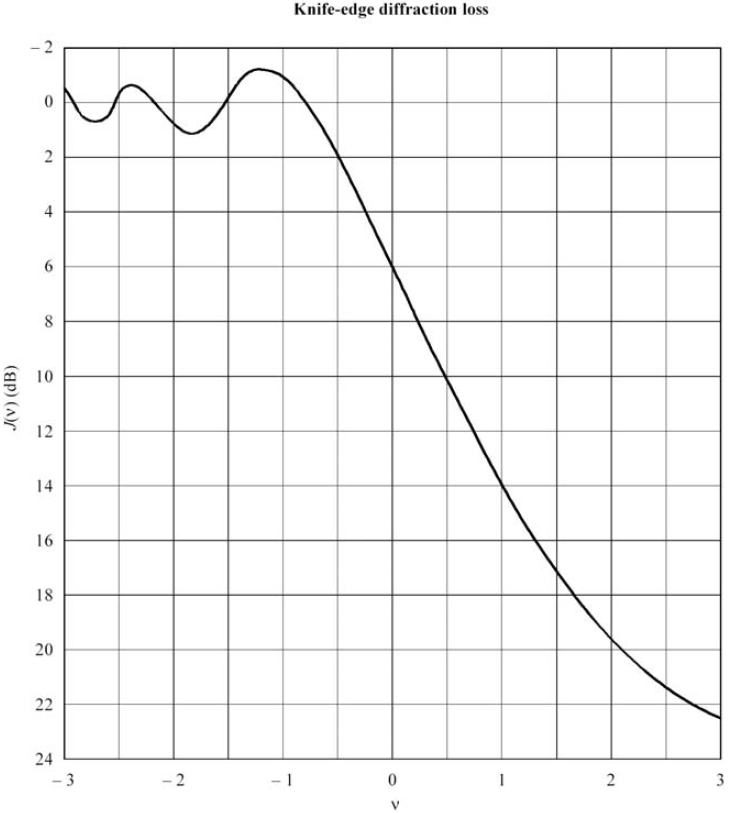
\includegraphics[scale=0.7]{figures/DiffractionLoss.PNG}
\caption{Loss due to diffraction. (figure 9 from \cite{ITU-R}, courtesy of ITU)}
\end{figure}

When $v=0$, the 1st Fresnel zone is 50\% blocked and the received signal loss is 6dB. 

\subsubsection{Single rounded-surface diffraction}
Sadly, most blockages encountered in the real world are not well-modeled by a knife-edge diffraction model, explained in the above section, because the tips dimensions which are bigger than the wavelength of the transmitted wave. A solution this, is to use the rounded-surface diffraction model, where the diffraction is treated as a cylinder, depicted on figure 2.10 below. 

\begin{figure}[h]
%\centering
\hspace{0.5cm}
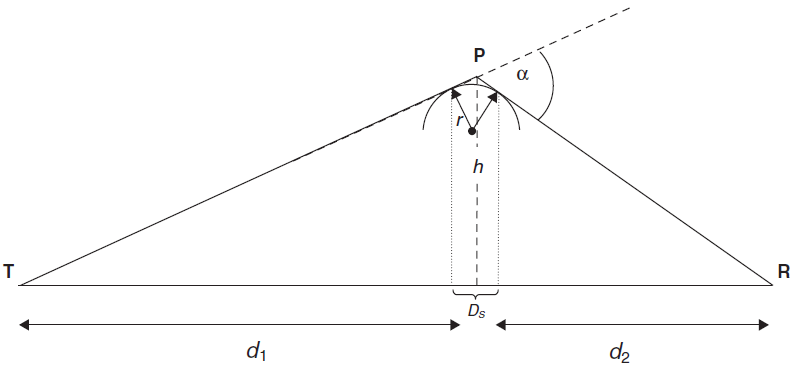
\includegraphics[scale=0.7]{figures/RoundedDiffraction.PNG}
\caption{Geometry for rounded-surface diffraction model\cite{RFpropagation} page 183}
\end{figure}

The diffraction from a rounded surface is determined by calculating the knife-edge diffraction and then computing the excess diffraction loss $L_{ex}$, due to the rounded surface. The excess diffraction loss is:

\begin{equation}
    L_{ex} = -11.7 \alpha\sqrt{\frac{\pi r}{\lambda}} dB
\end{equation}

where:

\begin{equation}
    \alpha = v\Big(\frac{\lambda(d_1+d_2)}{2d_1d_2}\Big)
\end{equation}

and r is estimated to be:

\begin{equation}
    r = \frac{2D_sd_1d_2}{\alpha(d_1^2+d_2^2)}
\end{equation}

Where $D_s$ is the extent of the diffraction surface. 

\subsubsection{Doppler spread}
Relative motion between the transmitter and receiver results in a Doppler shift\cite{DopplerShift} on the signal, where the entire spectrum is shifted in frequency. When multipath is combined with relative motion the radio wave may experience positive and negative Doppler shift, smearing or spreading of the signal frequency. This effect is called Doppler spread. The magnitude of the Doppler shift depends on the geometry of the signal path and the reflected signal path for multipath. The  \textit{Coherence Time} is defined as the time duration over which two received signal amplitude will be highly correlated.

\begin{equation}
    T_c \cong \frac{1}{f_m}
\end{equation}

where $f_m$ is the maximum Doppler shift:

\begin{equation}
    f_m = \frac{ v}{c}f_c
\end{equation}

where v, is the maximum velocity, c is speed of light and $f_c$ is the center frequency of the transmitted signal. If the signal bandwidth of the transmitter is much larger than twice the maximum Doppler shift the Doppler spread effect is negligible, this can be expressed as\cite{RFpropagation} page 199:

\begin{equation}
    f_{BW} >> 2 \cdot f_m
\end{equation}

\subsection{Absorption attenuation}
There are multiple phenomenons that can absorb a radio wave signal, some of them can easily be quantified and tested out, like loss through buildings, walls, windows and other physical objects, while other can only be calculated like atmospheric loss and rain and cloud losses. This section will shortly describe the losses behind these phenomenons compared to different frequencies, since it might be possible that they will influence the Link Budget when range tests are being conducted. 

\subsubsection{Concrete, glass, brick, fiberglass, etc}
There are different physical objects than can partially or fully block a radio wave. For this thesis, it only makes sense to look into walls and windows, since depending on where it is chosen to test the radio communication system there might be these obstacle standing in the way, therefore it is good a roughly estimate on how much they attenuate the signal. 

Appendix B \textit{Losses through building material} shows a list that has been conducted by a university student, Robert Wilson, at \textit{University of Southern California}. This list depicts all losses tested in a anechoic chamber (it is a room designed to completely absorb reflections from electromagnetic waves) for common building materials. The paper \cite{Magis} also states what the thickness of these materials are. For example the Fiberglass has a of 89mm and a reflection loss of around -39dB, which is a lot. DanSTAR will use fiberglass for the rocket hull, but the thickness will be no more than 2mm. Assuming the loss is linear with the thickness of the fiberglass, then it is around -1dB loss for 2mm fiberglass.

Another scientific paper has tested the loss through brick walls and windows\cite{ModernBuildings}. This test was conducted at frequencies spanning from 800MHz to 18GHz. In the article at page 5, figure 6, it is clearly possible to see that the higher the frequency the higher is the loss through the objects they have tested, although at some specific frequencies with the test object \textit{Windows MOB} the attenuation dips down again before going up. 

Depending on where the range test is going to be conducted for this thesis, it is important to include the above two articles in the link budget calculation, if it is piratically impossible to avoid the obstacles. 

\subsubsection{Vegetation}
It may happen that the range test will be conducted in such a way that there are foliage in the LOS path. This section presents a known model, which provide a estimate of the additional attenuation due to foliage that is within the LOS path. There are a variety of different models that depicts the loss from foliage. For this thesis only the most conservative one will be used, \cite{RFpropagation} page 135, shows both \textit{Weissberger's model} and \textit{Early ITU vegetation model}, in the book it can be observed that the \textit{Early ITU vegetation model} is the most conservative one, with the formula:

\begin{equation}
    L(dB) = 0.2F^{0.3}d_f^{0.6} dB
\end{equation}

where:

\begin{itemize}
  \item F is the frequency in Mhz
  \item $d_f$is the depth of the foliage along the LOS path in meters
\end{itemize}

\subsubsection{Terrain}
There are also multiple models that depicts the terrain loss, in this thesis the model form ITU will be used. The ITU terrain model is based on diffraction theory and provides quick means of determining a median path loss. The below figure 2.12, shows three plots of the expected diffraction loss due to terrain roughness vs the normalized terrain clearance. Curve B is the theoretical knife-edge diffraction curve, see section (2.5.2.3) \textit{Single knife-edge diffraction attenuation}. Curve D is the theoretical smooth-earth loss at 6.5 GHz using a 4/3 earth radius. The middle curve labeled $A_d$ is the ITU terrain loss model. Each of these models represents an excess terrain loss, beyond free-space loss, described in section (2.5.1) \textit{Free-space attenuation}. 

The ITU terrain loss model is given by:

\begin{equation}
    A_d = \frac{-20h}{F_1}+10
\end{equation}

where $h$ is the height difference in meters between most significant path blockage and the path trajectory. If the blockage is above the LOS path, then $h$ is negative. $F_1$ is the radius of the first Fresnel zone, see section (2.5.2.2) \textit{Fresnel Zone}, which is given by the formula:

\begin{equation}
    F_1 = 17.3 \sqrt{\frac{d_1d_2}{fd}}
\end{equation}

where:

\begin{itemize}
  \item $d_1$ and $d_2$ are the distances from each transceivers to the blockages in kilometers(see figure 2.8)
  \item d is the distance between the transceivers in Km
  \item f is the frequency in GHz
\end{itemize}

Equation (2.57) and (2.58) is from ITU's article \textit{Propagation data and prediction methods required for the design of terrestrial line-of-sight systems}\cite{ITUTerrain} on page 3. The $h/F_1$ is the normalized terrain clearance. This model is considered valid for losses above 15 dB, but can be used for as little as 6dB. The two other curves shown on figure 2.11, represent extremes of clear terrain and very rough terrain, thus the middle curve can be used to good guideline between the two extremes.  

\begin{figure}[h]
\centering
%\hspace{0.5cm}
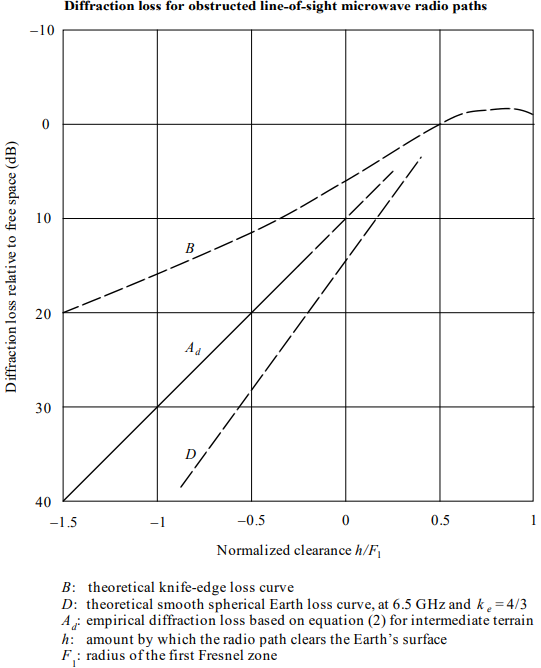
\includegraphics[scale=0.85]{figures/ITUTerrain.PNG}
\caption{Additional loss from terrain diffraction vs the normalized clearance model\cite{ITUTerrain} - page 4}
\end{figure}

\subsubsection{Atmospheric attenuation}
The atmosphere consists of gases, which absorb Rf waves at various frequencies. The gases of primary concern for microwave frequencies are oxygen and water vapor. Atmospheric attenuation depend upon pressure, temperature and water vapor content. For this reason the effect can very considerably with location, altitude and frequency. Modeling the attenuation of RF signal by atmospheric losses is a well known process that is explained in an article published by ITU, titled \textit{Attenuation by atmospheric gases}\cite{ITUAtmosphere} page 4 and 7. For radio links where the transmitter and receiver are at or near the same altitude, the atmosphere can be treated as constant over the path, thus it makes sense to characterize the absorption as a specific attenuation value having the unit dB/km. This attenuation will bee applied to the total LOS path. The expression for the loss due to atmospheric absorption is: 

\begin{equation}
    A = \gamma_ad dB
\end{equation}

where d is the LOS distance between the transmitter and receiver in km and $\gamma_a$ is the specif attenuation of the atmosphere in dB/km. It is a sum of the attenuation of water vapor and oxygen, since these are two biggest factors for system that ranges from 2-40Ghz, the formula is:

\begin{equation}
    \gamma_a = \gamma_o + \gamma_w
\end{equation}

While ITU gives formulas for these parameters, they are very long and tedious to evaluate in this thesis. Instead of calculating the attenuation, it is a common practice to use values extracted from a plots like on figure 2.12. This figure shows the absorption in dB/km for a given frequency, at near earth propagation (parallel to earth surface). 

\begin{figure}[h]
\centering
%\hspace{0.5cm}
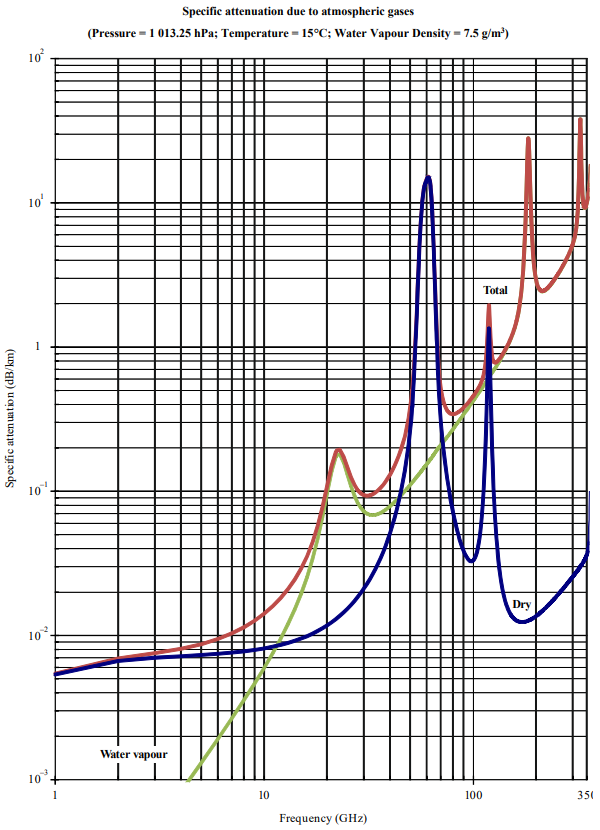
\includegraphics[scale=0.8]{figures/AbsorbsAtmosphere.PNG}
\caption{Additional loss due to atmosphere at near earth, courtesy of ITU\cite{ITUAtmosphere} - page 17}
\end{figure}

Figure 2.13 show the same as figure 2.12, but for a radio waves propagating vertically. This figure will be used in the Link budget, when the rocket is flying upwards and figure 2.12 will be used when the rocket is on the launchpad.

\begin{figure}[H]
%\centering
\hspace{-3cm}
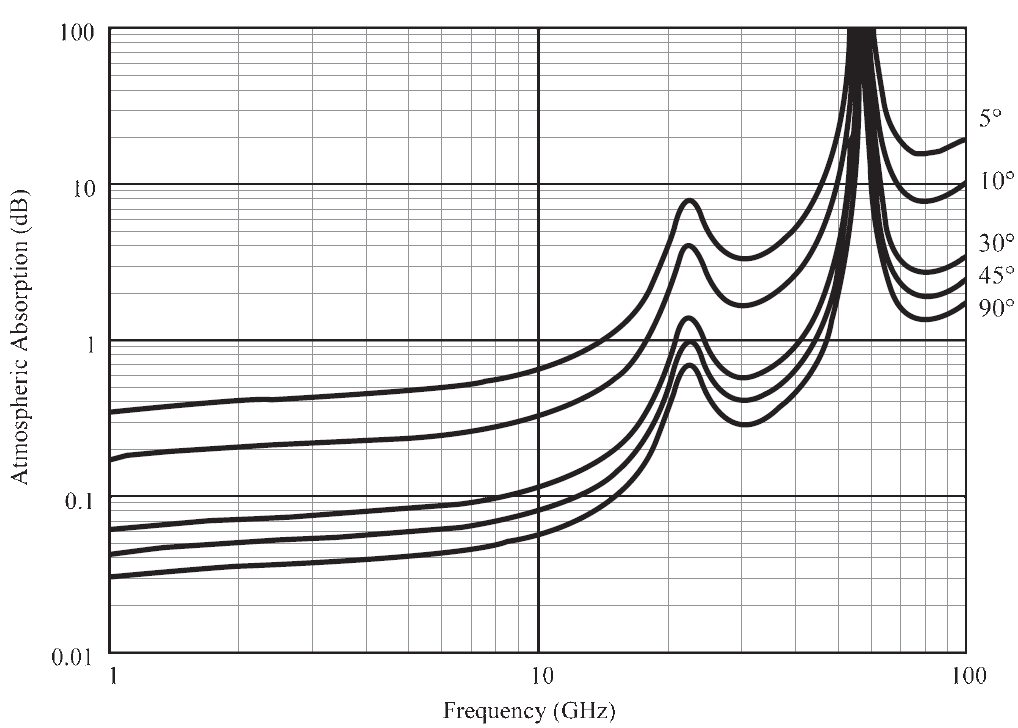
\includegraphics[scale=0.7]{figures/AbsorbsAtmosphereVertical.PNG}
\caption{Additional loss due to atmosphere at vertical propagation\cite{RFpropagation} - page 253}
\end{figure}

\newpage

\subsubsection{Rain and cloud attenuation}
When DanSTAR has to conduct a flight-test of its rocket, the test will certainly be done when it is not raining, since a lot of the ground equipment and the electronics in the rocket can malfunction. When it comes to testing only the telemetry system it will be a bad idea for the author of this report to conduct these tests when it is raining, since water and electronics does not go well together. Therefore, it will only make sense to implement rain attenuation in the link budget, when it seems to be absolutely necessary. A reference to an already well known rain attenuation model, done by the ITU is good enough for the thesis. Following the instruction on \cite{ITURain} on page 15, will return the rain attenuation in dB. Furthermore, the book \textit{Introduction to RF propagation} also has an explanation starting from page 224, which is also based on ITU's rain attenuation model.

When it comes to cloud attenuation, it makes sense to look in to the theory behind calculating the attenuation, since the rocket, on its way up, will go through clouds. ITU provides a recommended model for fog and cloud attenuation, see reference \cite{ITUCloud} page 4 formula (13), which is: 

\begin{equation}
    A = \frac{LK_t}{sin(\theta)} \quad dB \quad for \ang{90}\geq\theta\geq\ang{5}
\end{equation}

where:

\begin{itemize}
  \item $L$ is the total columnar liquid water in $kg/m^2$ estimated to be worst case $1kg/m^2$ based on \cite{ITUCloud} page 6. 
  \item $K_t$ is the specific attenuation coefficient in dB/km see figure 2.14
  \item $\theta$ is the elevation angle of the path
\end{itemize}

\begin{figure}[h]
\centering
%\hspace{-3cm}
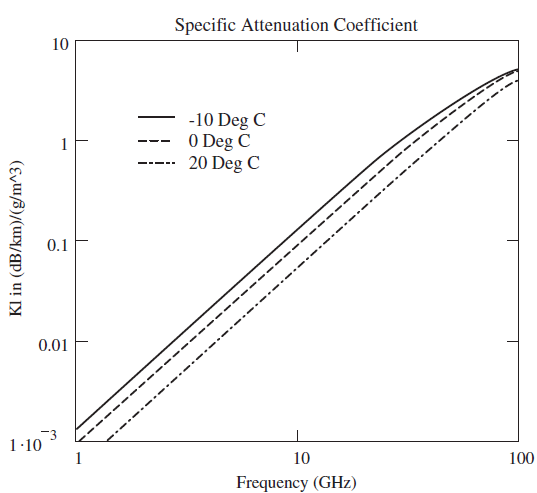
\includegraphics[scale=0.7]{figures/Kl.PNG}
\caption{specific attenuation coefficient\cite{RFpropagation} - page 127}
\end{figure}

\subsection{Coaxial Cable losses}
A coaxial cable cunducts electrical signal using an inner conductor, usually made of copper, surrounded by an insulating layer, which is enclosed by a metallic shield. The coaxial cable is protected by a outer insulating jacket. The advantage of a coaxial cable is that the signal is restricted by the dielectric layer, with little leakage outside the shield. This property of the coaxial cable makes it a excellent choice for RF signal that cannot tolerate interference from the environment\cite{CoaxialCable}, see figure 2.15. A Coaxial cable, can come with different materials resulting in different properties. Some cables are simi-rigid, witch means they are hard to bend, but once bent they will contain their shape, these cables usually have lower losses, other cables are thinner easier to bend, but the losses a higher. Most coaxial cables has an impedance of either $50\Omega$ or $75\Omega$ and the losses (in dB) pr unit length is varies from cable to cable, Wikipedia has a good list of coaxial cables, depicting parameters such as: impedance, dielectrics, size, shielding and losses (in dB) pr unit length (dB/100feet), see reference \cite{CoaxialCable}, section \textit{Standards}

\begin{figure}[h!]
\centering
%\hspace{-3cm}
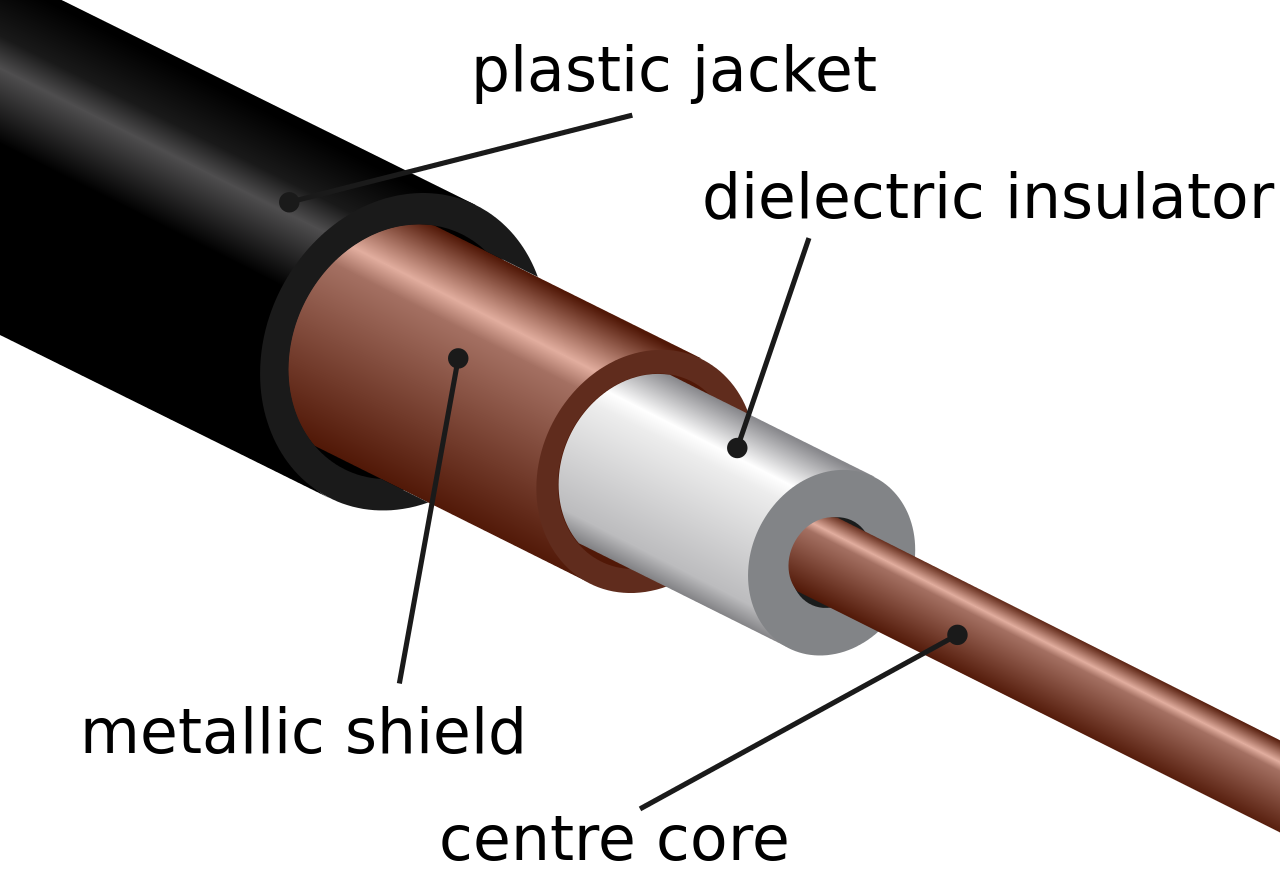
\includegraphics[scale=0.15]{figures/CoaxialCable.png}
\caption{Coaxial cable\cite{CoaxialCable}}
\end{figure}

\subsection{Connector losses}
In this thesis mainly SMA connectors will be used. Like a coaxial cable, the SMA connector has a inner core usually gold plated, surrounded by a dielectric material, contained inside a metal housing that is gold plated. The metal housing is the outer conductor, see figure 2.16. 

\begin{figure}[h!]
\centering
%\hspace{-3cm}
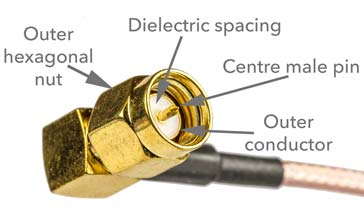
\includegraphics[scale=0.6]{figures/SMAConnector.jpg}
\caption{SMA connector{SMAConnector}}
\end{figure}

There are many types and shapes for a SMA connectors, this reference \cite{SMAConnectorLosses} (page 102) shows the losses for a given type of a SMA connector. However, what needs to be noted is that the datasheet is from a company \textit{Tyco Electroncs} this means the results can only guaranteed if one buys SMA connectors from them. 

\section{Thesis specific losses}
Beside the losses described in the sections above, there are also thesis specific losses. These losses only occurs, because the transmitting antenna is mounted on a rocket, which can accelerate over 3G, and travel at a speed above 400m/s. Furthermore, since the rocket has fins to aerodynamically stabilize it, the mounting of the fins will never be 100\% symmetric, therefore they will induce a torque around its z-axis, which will make the rocket spin around itself, this phenomenon can introduce a huge loss. The below section will clarify how these losses occurs and also how big of a problem they are.

\subsection{Antenna misalignment attenuation}
In applications where directional antennas are used, both on the transmitter and receiver side, it is important that the antennas point towards each other. For example in a static setup, where WiFi in a community is being extended from one house to another, the antennas has to point at each other to allow for the best connection strength.  

For this thesis, it is assumed the above to be true for the rocket only when the rocket is on the launch rail, ready to be fired, but as soon as the rocket starts to fly, the system will transitions from a static setup to a dynamic setup where the operator on the ground has to track the rockets movements. Depending on what type of antenna is being used (directional or omnidirectional) in the rocket, there will certainly be antenna alignment losses.

Figure 2.15 depicts the problem, with two directional antennas. For an omnidirectional and a directional antenna setup, the problem will still occur but it will not be as problematic. % for more information about how antennas work see section 2.7 ....   

\begin{figure}[h]
\centering
%\hspace{-3cm}
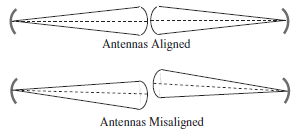
\includegraphics[scale=1]{figures/AntennasAlignment.PNG}
\caption{Antenna misalignment loss - in courtesy of John S. Seybold  \cite{RFpropagation} - page 63}
\end{figure}

It is hard to  quantify the size of the misalignment loss in dB, since it depends on how good the operator is at aiming towards the rocket. If, on the other hand, the on ground system is automatically capable of tracking the rocket, the antennas on the ground will have to be purposely pointing away from the rockets antenna peak beam. This purposely misalignment of the antenna is very small and can be combined with the RSSI value to allow for automatically tracking of the rocket. %where should we write about how this is done? 

\subsection{Polarization mismatch}
For a static radio communication setup, as long as the antennas on both the transmitter and receiver side are placed with the same polarity, there will be no losses, due to polarization mismatch. For example if a linear antenna (quaterwavve monopol antenna, see section 2.7.2 \textit{Quaterwave monopol}) is horizontally mounted on the rocket, which is stationary on the launch pad, and a linear antenna (yagi antenna, see section 2.7.6 \textit{Yagi-uda and cross yagi-uda}) is horizontally mounted on the ground (mission control), then there will be no loss, since both antennas will be radiating and receiving with the same polarity - horizontally. But it is different when everything becomes dynamics, where the rocket is flying in the air. if it Suddenly starts to tumble (because of aerodynamic reasons), then the linear antenna mounted horizontally on the rocket, might not be horizontally looking anymore from the perspective of the receiver. This will introduce huge losses up to -20 dB. Theoretically it is infinity loss, but in reality the polarity might change because of multipath cases, allowing for some signal to reach the ground antenna with the same polarity or a slant polarity. To avoid the above problem, a helical antenna can be used as ground antenna, which will neglect the problem, since a helical antenna does not care about the polarity. Although using a helical antenna on ground and a linear antenna on the rocket, will introduce a total loss of -3dB. This payoff is much better than losing -20dB, due to linear antennas being used on both sides.   

%%For more theory about polarization please read section ....... to fully understand the scope of the problem. See the tables... 

\subsection{Package loss due to high axial rotational speed of the rocket}
Another loss that is specific to this thesis, is the phenomenon where the rocket itself is obscuring the transmitted radio signal. As explained above, the rocket will have a tendency to rotate around it z-axis, if the rotational speed of the rocket is greater than speed it takes to transmit a single package of data down to earth, then it is possible to experience losses since the transmitting antenna will rotate to the other side where there is no ground antenna to receive the signal, effectively the rocket will block the transmitted radio wave, due to it standing in the way of itself. On figure 2.16 it is observed that there are 3 antennas, 1 on the ground and 2 on the rocket - a right and a left antenna. The actual rocket will have 3 antennas spaces 120-degrees from each other, but for the sake of simplicity a 2D drawing is enough. The rocket is rotating around itself at a speed that is quite hard to estimate, it can be anywhere from 5Hz to 30Hz. The case is, when the right antenna is transmitting and the rocket is stationary, then everything is good since the receiver antenna is in line-of-sight with the right antenna. The moment the rocket lifts off, the small misalignment (which is mechanically hard to avoid) of the fins of the rocket will induce a torque, that in return will make the rocket rotate. When the rocket turn half revolution the right antenna will then be on the left side an obscured from the hull of the rocket. Depending on what is inside the rocket and what material the hull is made out off the signal loss can be huge. For worst-case scenario, it is assumed to be -20dB, practically meaning the signal will be lost. Once the rocket rotates another half revolution then the obscured antenna will go back to its starting point, where the signal is highest. Now, what is experienced in reality is a sinusoidal wave, where the amplitude of the wave is the value of RSSI, and the frequency of that wave is the rotational speed of the rocket, what is meant here is that we will not experience a sudden drop of -20dB but a gradual drop towards -20dB, depending on the rotational speed. 

\begin{figure}[h]
\centering
%\hspace{-1cm}
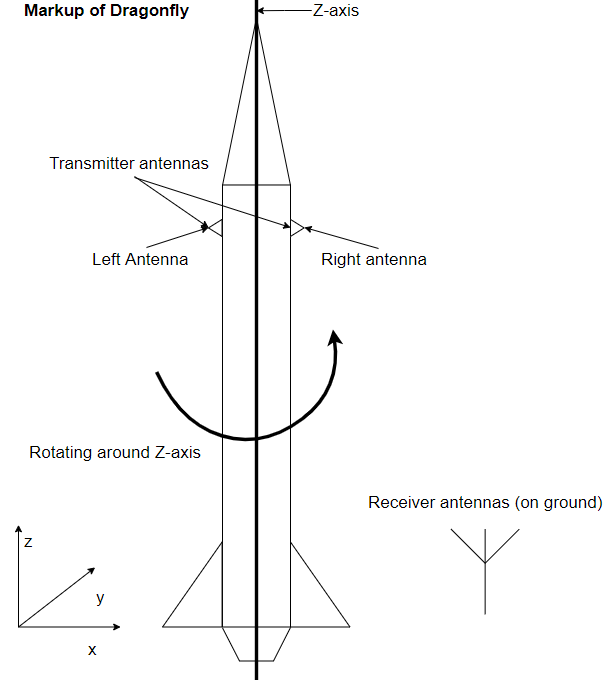
\includegraphics[scale=1]{figures/RocketShading.PNG}
\caption{Markup of Dragonfly, showcasing the mounted antennas on the rocket and the ground antenna}
\end{figure}

From a simple calculation it is people to figure out what the maximum rotational speed is for fixed sized packet size, before the antenna is on obscured by the rocket, the time it takes to send a package, also called time on-air, is given by the formula:

\begin{equation}
    T_{OA} = \frac{packet\ size [bit]}{air\ data\ rate [\frac{bit}{s}]}\ [s]
\end{equation}

Where the packet size is in [bits] and air date rate is in [bit/s]. Both values can be programmed to be a fixed value depending on what the datasheet is saying for a given transceiver. 

The frequency is given by:

\begin{equation}
    f = \frac{1}{T}\ [Hz]
\end{equation}

Where $T$ is the period in seconds, denoted s.

Since the transmitter only has a half rotation where it can transmit data before it gets obscured by the rocket, then the goal is to make sure that the following inequality is true:

\begin{equation}
    \frac{T}{2} \geq T_{OA}
\end{equation}

What can be deduced from the above equations (2.63) and (2.64) is that to uphold the inequality (2.65), one can lower the packet size or increase the air data rate or decrease the rotational speed of the rocket (measured in Hz). Increasing the air data rate, lowers the sensitivity of the transceiver, which decreases the link margin (see section 2.8.1 \textit{Link budget margin}) this happens because the bandwidth increases to accommodate for the higher data rate, which will allow for more noise into the receiver, reducing the sensitivity margin. Unless DanSTAR build an counter rotational system in the rocket, the axial rotation cannot be controlled therefore this parameter is fixed. The final and easiest variable to change is the packet size, since the downside of it only the need to of transmitting more packages to accommodate for the data produced by the rocket. 

Some transceivers has a function that allow for dynamic package lengths, this can be combined with the navigational system that can calculate the rotational speed while the rocket is flying, using the following equation:

\begin{equation}
    \omega = \frac{2\pi}{T} = 2 \pi f
\end{equation}

where $\omega$ is the angular velocity in $[\frac{radians}{s}]$

When combining the above equation with the dynamic package size function, we can create a model in which the package size dynamically changes depending on what the navigational system has calculated the rotational speed of the rocket to be. In this way the computer can figure out, by itself, what the optimal package size should be.

\section{Antenna in general}
For any type of a point-to-point radio communication system it is important to understand how antennas operate. Antennas are used to radiate and receive electromagnetic energy and they are a essential prerequisite for being able to calculate a good link budget.

This theory section will go through the basic of how antennas work and the different type of antennas that exists, although there are many, only thesis specific antennas will be described.

\subsection{Isotropic antenna}
An isotropic antenna, is an theoretical ideal antenna that radiates or receives equally in all direction, with a spherical pattern. Isotropic radiators are used as a reference radiators with which other sources are compared against, for example when determining the gain of a practical antenna. Se figure 2.17, depicting the isotropic radiator. Since the isotropic radiator is radiating equally in all direction the directivity of this theoretical antenna is 1 and the efficiency is 100\% meaning the gain is 0 dBi. Since most practical antennas are referenced to an isotropic antenna, the gain of these practical antennas are in the unit of dBi. Some manufactures reference them to a dipole antenna where the unit then becomes dBd. see section 2.1.3 \textit{what is dB/dBi/dBd/dBW/dBm?}.  

\begin{figure}[h]
\centering
%\hspace{-3cm}
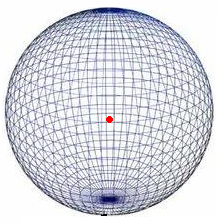
\includegraphics[scale=1.3]{figures/Isotropic.png}
\caption{Isotropic radiator - a point in space radiating equally in all direction in a spherical pattern}
\end{figure}

\subsection{Directivity, efficiency and gain}
Any practical antenna will exhibit some directivity in its radiation patters, even the simplest types such as dipole antennas. figure 2.18 is a simple picture that explains the concept of antenna directivity. The balloon 2.18(A) that is blown up to it usual - close to - spherical shape, represents the "reference" isotropic antenna. Squeezing the balloon in the middle 2.18(B) produces a dipole-like pattern (see section 2.6.2 \textit{Dipole}), a figure 8 pattern, where the peak level is at the top and bottom, lager than the isotropic reference balloon. Also see figure 2.3, further up in section 2.1.3 \textit{what is dB/dBi/dBd/dBW/dBm?}. Next, squeezing the balloon close to the bottom in figure 2.18(C) produces a pattern with even more gain in the top compared to the reference, this could be a high gain antenna, such as a yagi or a helical antenna. The directivity of an antenna is defined as the ratio of the peak power density at distance, d, to the average power density at d, as seen below:  

\begin{equation}
    D = \frac{P}{\frac{P_T}{4 \pi d^2}} = \frac{P}{P_{av}} 
\end{equation}

where:

\begin{itemize}
  \item $D$ is directivity.
  \item $P$ is power density at its maximum point on the surface of the sphere.
  \item $P_T$ is the power applied to the antenna terminals.
  \item $4 \pi d^2$ is the surface area of a sphere with radius d.
  \item $P_{av}$ is average power density, given by $\frac{P_T}{4 \pi d}$.
\end{itemize}

As stated above the directivity of an isotropic antenna is 1, when the antenna losses (or in other words the efficiency) are included in the directivity, then we can calculate the gain of the antenna, with the formula:

\begin{equation}
    G = \epsilon_r D = \frac{P_r}{P_i}\cdot\frac{P}{P_{av}} \quad dBi
\end{equation}

where $\epsilon_r$ is antenna efficiency, which can be written as $P_r$ power radiated over $P_i$ power input.

What is important to state here, is that the gain of a given antenna only has the antenna efficiency included in the calculation, as equation (2.68) shows. It does not include the impedance mismatch loss, see section 2.5.7 \textit{Impedance matching loss}. Furthermore, the higher the gain the lower the field-of-view of the antenna is. This again can be visualized with the balloon analogy. Imagine if the balloon was squeezed with multiple hands, from the sides and behind it will only be able to expand forward this creates a much thinner main lobe, thus the gain will be increased tremendously but the field-of-view will be significantly reduced, since the main lobe is so thin. See also section 2.5.4 \textit{Radiation pattern}.   

\begin{figure}[h]
\centering
%\hspace{-3cm}
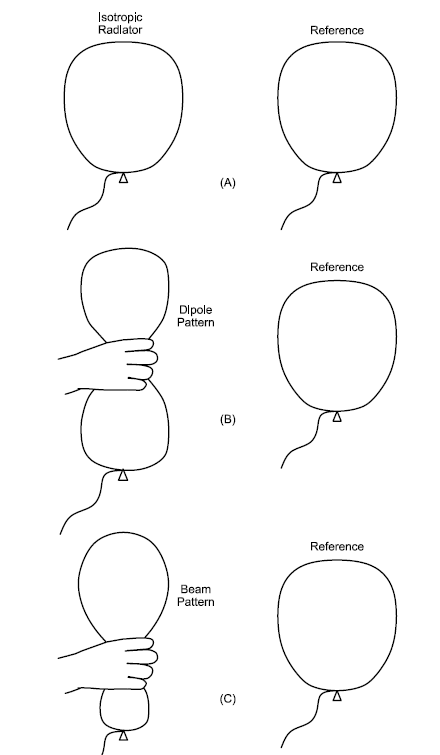
\includegraphics[scale=0.8]{figures/BalloonDirectivity.PNG}
\caption{Demonstration of antenna patter gain with balloons - courtesy to the ARRL book, see reference: \cite{ARRL} - chapter 2 page 10}
\end{figure}

\newpage

\subsection{E-plane and H-plane}
For a linearly polarized waveguide antennas, two reference planes exists, a E-plane and a H-plane. These two planes can be used to characterize the radiation of an antenna, see section 2.5.4 \textit{Radiation pattern}.

For a linearly-polarized antenna the E-plane contains the electrical field vector and the direction of maximum radiation. The E-plane determines the polarization of an antenna or orientation of the emitted radio wave, see section 2.5.5 \textit{Polarization} to understand what polarization is. For a horizontally polarized antenna, the E-plane usually coincide with the Horizontal/azimuth plane over ground. 

For the same type linearly polarized antenna, the H-plane is the magnetic field vector, and the direction of maximum radiation. This plane is perpendicular to the E-plane and coincides with the elevation plane over ground, see figure 2.19 for the E and H-plane. 

\begin{figure}[h]
%\centering
\hspace{-0.5cm}
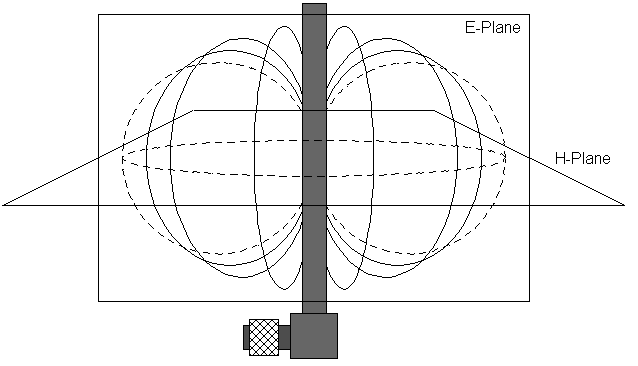
\includegraphics[scale=0.7]{figures/EH_Plane.png}
\caption{The E and H-plane depicted on a sleeved dipole antenna \cite{EH-plane}}
\end{figure}

\subsection{Radiation pattern}
The radiation pattern of an antenna defines the variation of the power radiated by an antenna as a function of the direction away from the antenna, by other words it is a graphical depiction of the gain of the antenna versus angle. The radiation pattern is always described for the far field region of the antenna, see section 2.5.6 \textit{field region}, where the gain is a function of the azimuth and elevation angles only. Figure 2.20 shows this graphical view of the radiation pattern for a dipole antenna, where the gain is plotted in dB.Figure 2.21 show the gain of a 2-dimensional cut for both the horizontal and vertical plane. 

The radiation pattern on the left is the azimuth plot. it is a function of the azimuth angle for a fixed polar angle (90-degrees off the z-axis,which is parallel with the antenna on figure 2.20). Since the radiation pattern in figure 2.20 is symmetrical around the z-axis, this plot appears as a constant in figure 2.21a

The radiation pattern on the right, figure 2.21b, is the elevation plot, which represent the plot of the radiation pattern as a function of the angle measured off the z-axis (for a fixed azimuth angle). The gain becomes maximum when the angle is perpendicular to the antenna, that is 90 and 180 degrees.

Figure 2.20 and 2.21 was simulated in the program 4nec2\cite{4nec2}, see section 3 \textit{Simulation}. 

\begin{figure}[h]
\centering
%\hspace{-1cm}
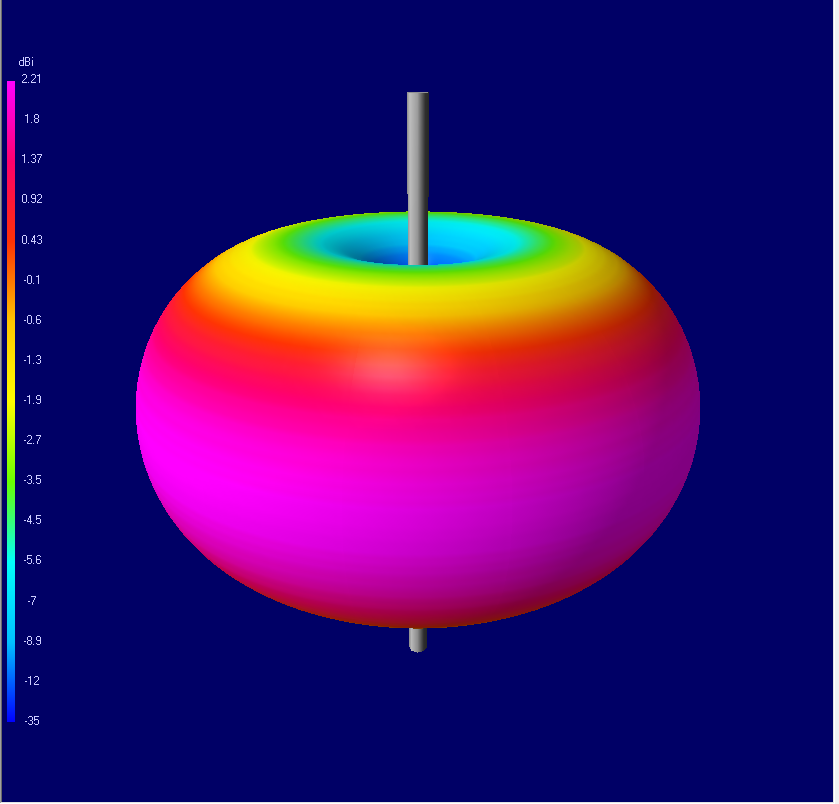
\includegraphics[scale=0.5]{figures/DipoleAntennaRad.PNG}
\caption{A 3-dimensional depiction of the radiation pattern for a dipole antenna in free-space}
\end{figure}

\begin{figure}[h!]
  \centering
  \begin{subfigure}[b]{0.49\linewidth}
    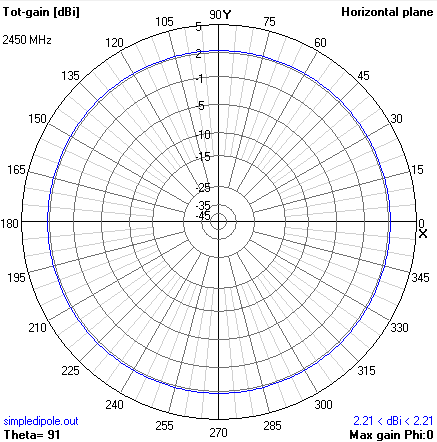
\includegraphics[width=\linewidth]{figures/HorizontalRad.PNG}   \caption{Total gain for Horizontal plane (azimuth) of a dipole antenna }
  \end{subfigure}
  \begin{subfigure}[b]{0.49\linewidth}
    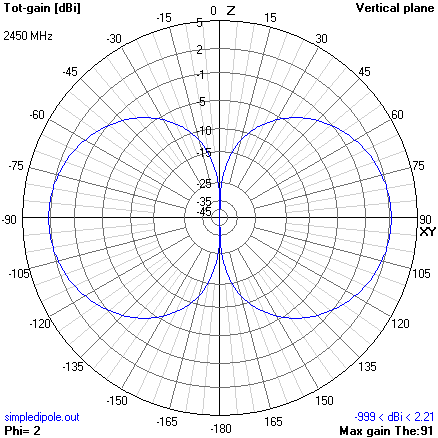
\includegraphics[width=\linewidth]{figures/VerticalRad.PNG}
    \caption{Total gain for vertical plane (elevation) of a dipole antenna}
  \end{subfigure}
  \caption{A 2-dimensional cut of the radiation pattern for a dipole antenna}
\end{figure}

Figure 2.20 shows that the dipole antenna is a omnidirectional antenna, meaning it is radiating equally in all direction in the horizontal plane, whereas figure 2.22 and 2.23 shows the radiation pattern of a helix antenna, where the radiation is focused towards a point. What can also be seen on figure 2.22 and 2.23 is the side lobes around the main beam, this means that not all of the energy is emitted "through" the main beam, but some goes to the side lobe, which make the antenna less effective (see next subsections). Furthermore, the helical antenna is simulated with real ground plane, acting as a reflector, whereas figure 2.20 is in free-space, see section 2.6.3 \textit{Helical} for more information about directed antennas. 

\begin{figure}[h]
\centering
%\hspace{-1cm}
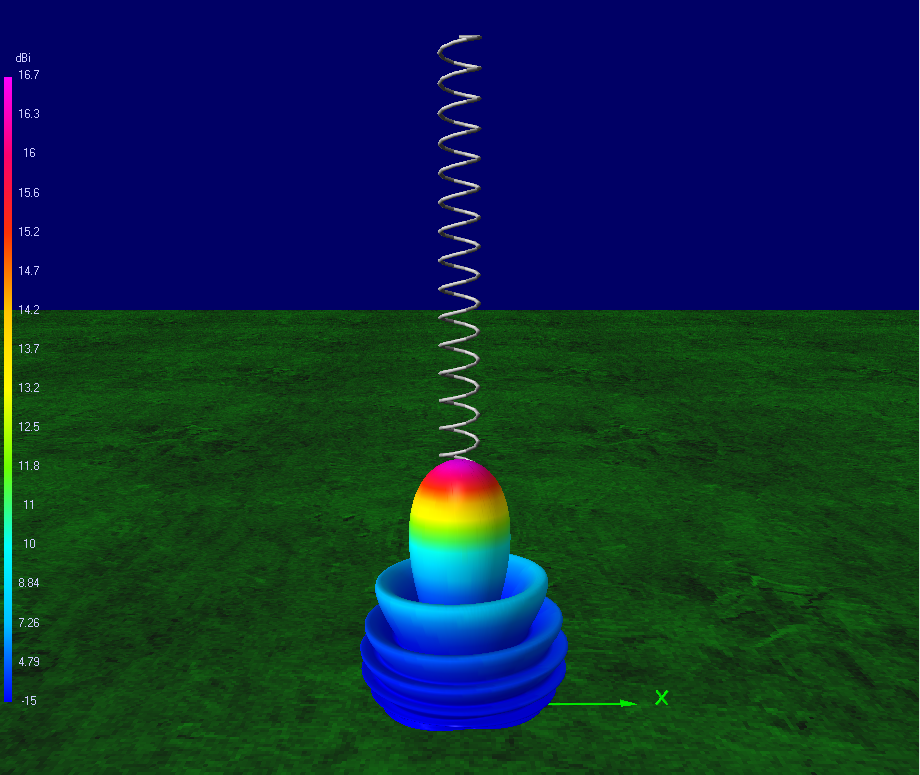
\includegraphics[scale=0.45]{figures/HelixRad.PNG}
\caption{Radiation pattern for a helix antenna - real ground plane }
\end{figure}

\begin{figure}[h]
\centering
%\hspace{-1cm}
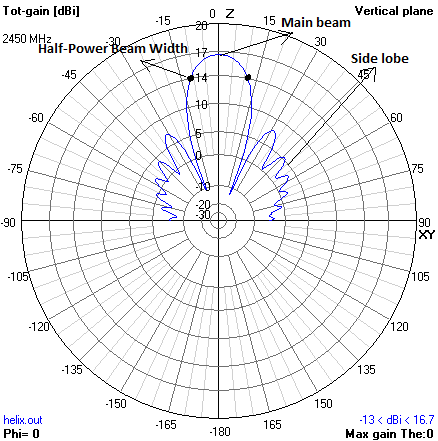
\includegraphics[scale=0.7]{figures/HelixVerticalrad.PNG}
\caption{A 2-dimensional cut of the radiation pattern for a dipole antenna }
\end{figure}

Figure 2.23 also show the type of lobes that exists for a directive antenna. There are 2 important lobes, the main lobe and the side lobe. Furthermore, there is the Half-power beam width, this is where the angular separation, in which the magnitude of the radiation pattern decreases by 50\% (or -3dB) from the peak of the main beam. On figure 2.23 it can be seen that the pattern decreases to -3dB at -10 degrees and 10 degrees, hence the is $HPBW = |-10|+10 =20 degrees$, this information can be used determine how much the receiver end can diverge away from the transmitter end, before the loss is greater than -3dB. 

\subsection{Field region}
The antenna radiation field is divided into 4 principle regions, where the characteristics of the radiated wave are different. While these regions are not firm boundaries, they provide some insight to the actual radiated field as a function distance from the antenna. Figure 2.24 depicts these regions.

\begin{figure}[h]
%\centering
\hspace{-1.5cm}
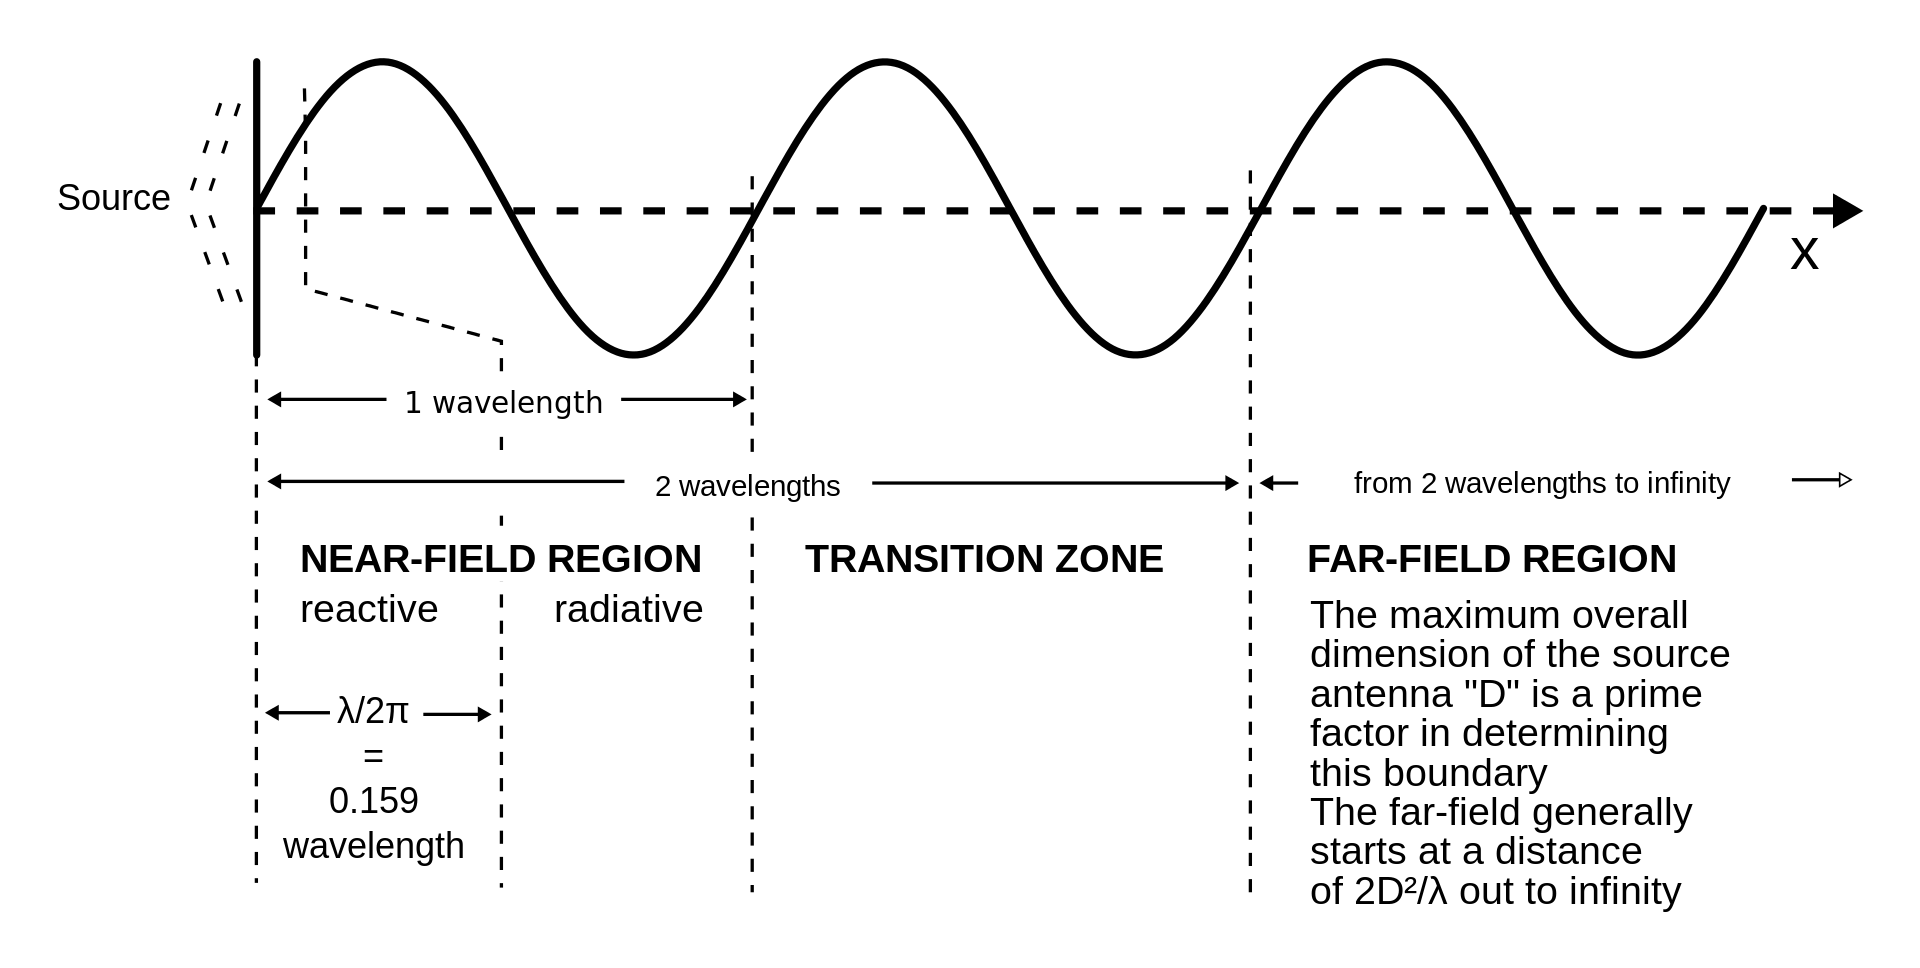
\includegraphics[scale=0.25]{figures/FieldRegions.png}
\caption{Field regions}
\end{figure}

\subsubsection{Far-field region}
The far-field region is the most important region, as this determine the antenna's radiation pattern, described in the section above. Antennas are use to communicate wirelessly from long distances, so this is the region of operation for most antennas. The far-field region is far from the antenna, as one might suspect. In this region, the radiation pattern does not change shape with distance (although the fields still die off as $\frac{1}{r}$). This region is dominated by the radiated fields, with E- and H-planes being orthogonal to each other and in phase. The far-field region is defined for distances $r$, such that 3 condition must be satisfied:

\begin{equation}
    r > \frac{2D^2}{\lambda}
\end{equation}

\begin{equation}
    r >> D
\end{equation}

\begin{equation}
   r >> \lambda
\end{equation}

where $D$ is the largest linear dimension of the antenna, and $\lambda$ is the wavelength. The first and second equation ensure that the power radiated in a given direction from distinct parts of the antenna are approximately parallel. This makes the far-field region behave like plane wave. The third condition is due to the antenna having reactive fields (see reactive near-field below) that have E-fields and H-fields die off with distances as $\frac{1}{r^2}$ and $\frac{1}{r^3}$. This is due to the fact that the magnetic field strength is proportional to the inverse-cube of the distance $r$, and electric field strength is proportional to inverse-square of distance $r$, thus the third condition ensures that these near field are gone, such that only the radiating field is dominant, which fall off with distance as $\frac{1}{r}$\cite{AntennaThoryFieldRegion}. 

\subsubsection{Transition zone}
The transition zone is between the near and far field regions and extends over the distance from one to two wavelength from the antenna. In this region, near-field dies out and ceases to be important, thus leaving the far-field effects to be dominant. 

\subsubsection{Radiating near-field region}
The radiating near-field region is also called the Fresnel region, since it is between the reactive near-field region and the far-field region and defined as:

\begin{equation}
    0.62 \cdot \sqrt{\frac{D^3}{\lambda}} < r < \frac{2D^2}{\lambda}
\end{equation}

Unlike far-field region the shape of the radiation pattern in the radiating near-field may vary with distance. Depending on the value $r$ and $\lambda$ this field may or may not exists, that is why this region is sometimes a part of the transition zone.   

\subsubsection{Reactive near-field region}
In the close vicinity of the antenna, the reactive near field is the most dominant factor. In this region the fields are predominately reactive fields, which means E- and H-plane are orthogonal to each other but are 90 degrees out of phase. In general any objects within this region will result in coupling with the antenna and distortion of the ultimate far-field antenna pattern. This phenomenon is used in the music instrument \textit{Theremin}\cite{Theremin}. Below is the condition for the reactive near-field region.

\begin{equation}
   r < 0.62 \cdot \sqrt{\frac{D^3}{\lambda}}
\end{equation}

\subsection{Polarization}
To avoid making this section too heavy and tedious to read through it is best to minimize any electromagnetism theory, and rather using graphical visualization to explain the theory behind polarization. For this a software program called Emanim\cite{EMANIM} is recommended to download and try out. All the figures below, will come from this software. If the reader wants the detailed theory, it is advised to read section 3.5 \textit{Antenna Polarization} in the book \textit{Introduction to RF Propagation} by John S. Seybold - page from 55 to 62.\cite{RFpropagation}.

Polarization is one of the fundamental characteristics of any antenna. Polarization is defined in the far-field region, see section 2.5.5.1 \textit{Far-field region}, of the antenna and is the orientation of the plane, by which the electrical field (E-plane) portion of the propagated wave is derived from. In the far-field region, the electrical field (E-plane), magnetic field (H-plane) and propagation direction vectors are all mutually orthogonal and in phase. This permits a complete characterization of a wave by describing the electrical field vector and the direction of propagation.

Most antennas and electromagnetic waves have either linear polarization (vertical or horizontal) or circular polarization, which can be right-hand or left-hand or elliptical Polarization. 

\subsubsection{Linear polarization}
A linear polarized antenna can both be in the vertical or horizontal position, relative to ground. An antenna is said to be linear polarized when the E-field is either oscillating forth and back in the x-axis (horizontal position) or in y-axis(vertical position). See figure 2.25 and 2.26 for vertical and horizontal polarization. 

\begin{figure}[h]
\centering
%\hspace{-1.5cm}
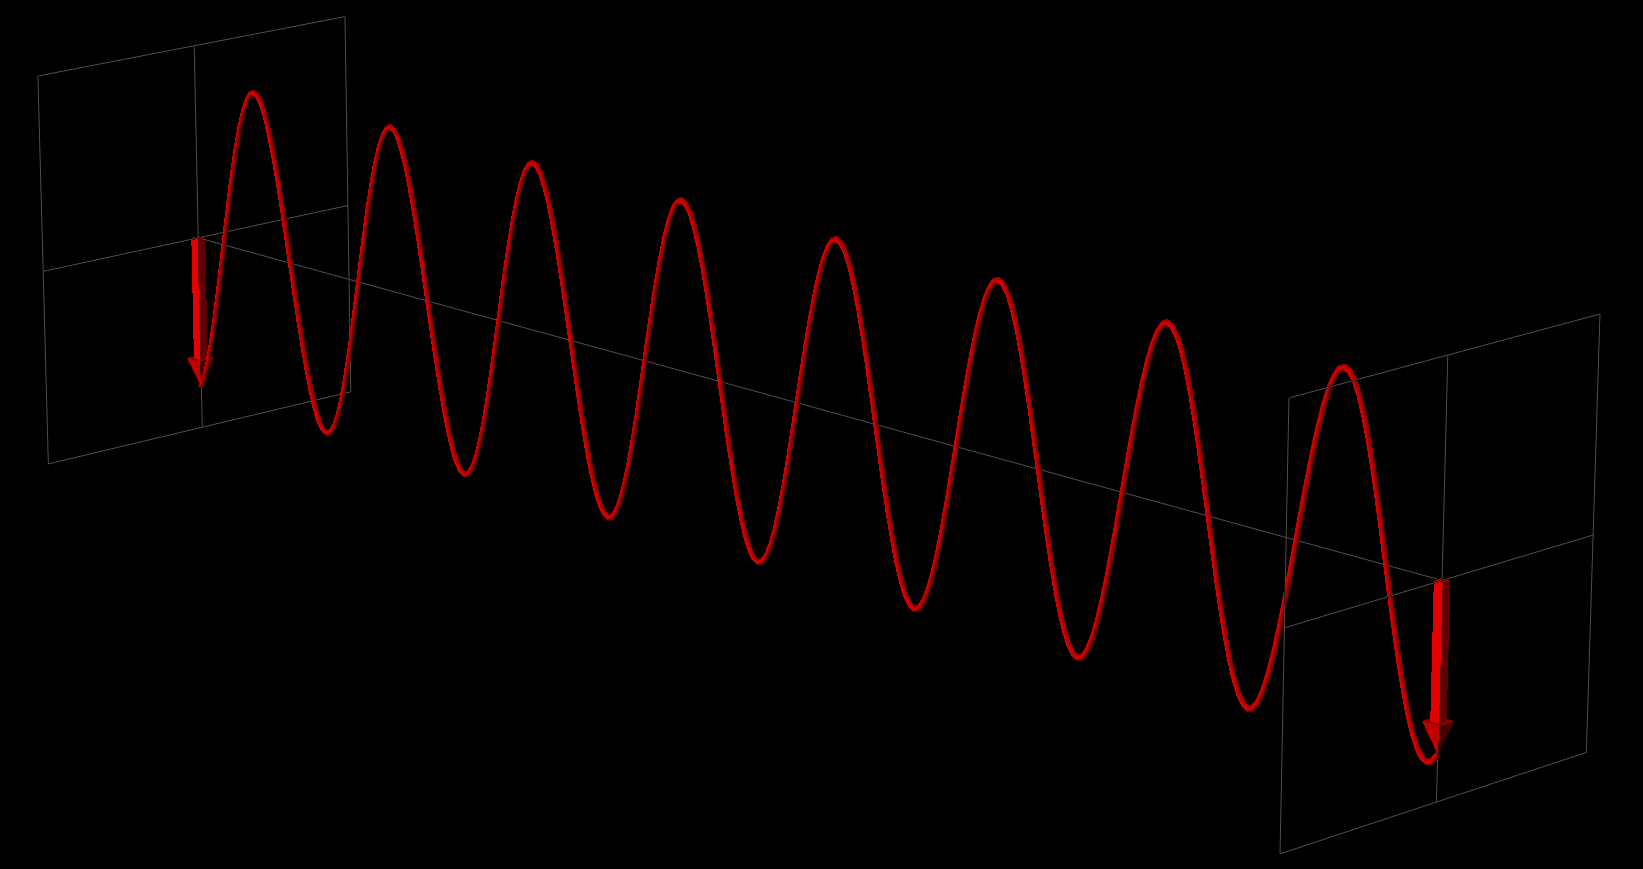
\includegraphics[scale=0.25]{figures/VerticalPolarization.PNG}
\caption{Vertical polarization}
\end{figure}

\begin{figure}[h]
\centering
%\hspace{-1.5cm}
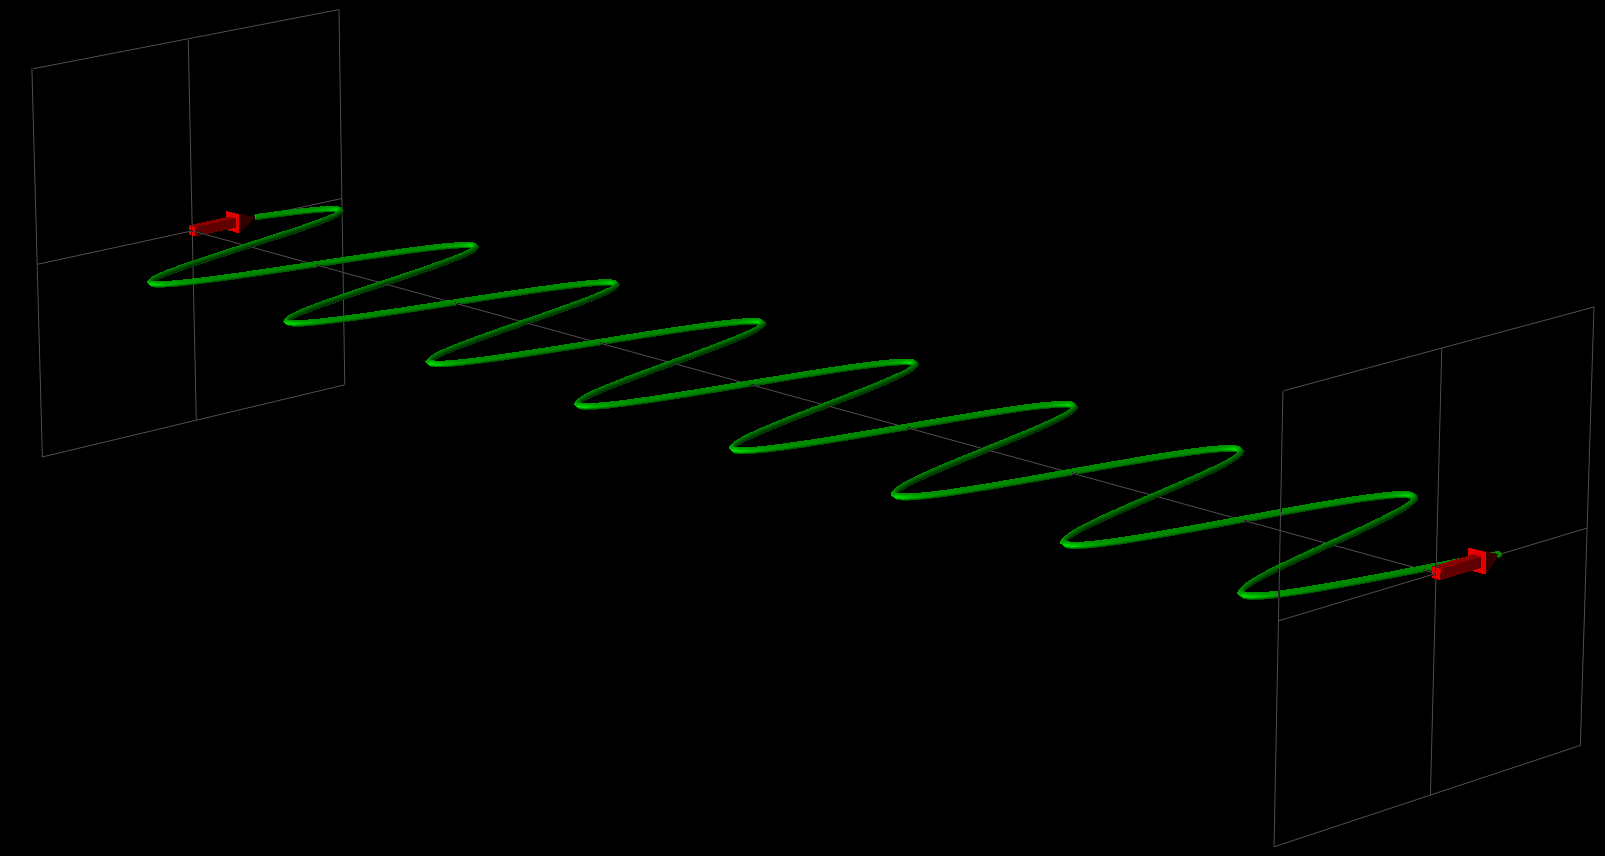
\includegraphics[scale=0.25]{figures/HorizontalPolarization.PNG}
\caption{Horizontal polarization}
\end{figure}

\subsubsection{Circular polarization}
When the x and y components of the electrical field is oscillating forth and back in their x- and y-axis while being 90 degrees out of phase and having the equal magnitude, the E-field will rotate in a circle, see figure 2.27. The have circular polarization, the following criteria  must be met:

\begin{itemize}
  \item The E-field must have two orthogonal components.
  \item The E-field's orthogonal components must have equal magnitude.
  \item The orthogonal components must be 90 degrees out of phase.
\end{itemize}

Circular polarization can a occur in tow forms, \textbf{Right hand circularly polarized} (RHCP) and \textbf{Left hand circularly polarized} (LHCP). This is important to note, since the transmitter and receiver must have the same polarization in order to avoid huge losses. 

\begin{figure}[h]
\centering
%\hspace{-1.5cm}
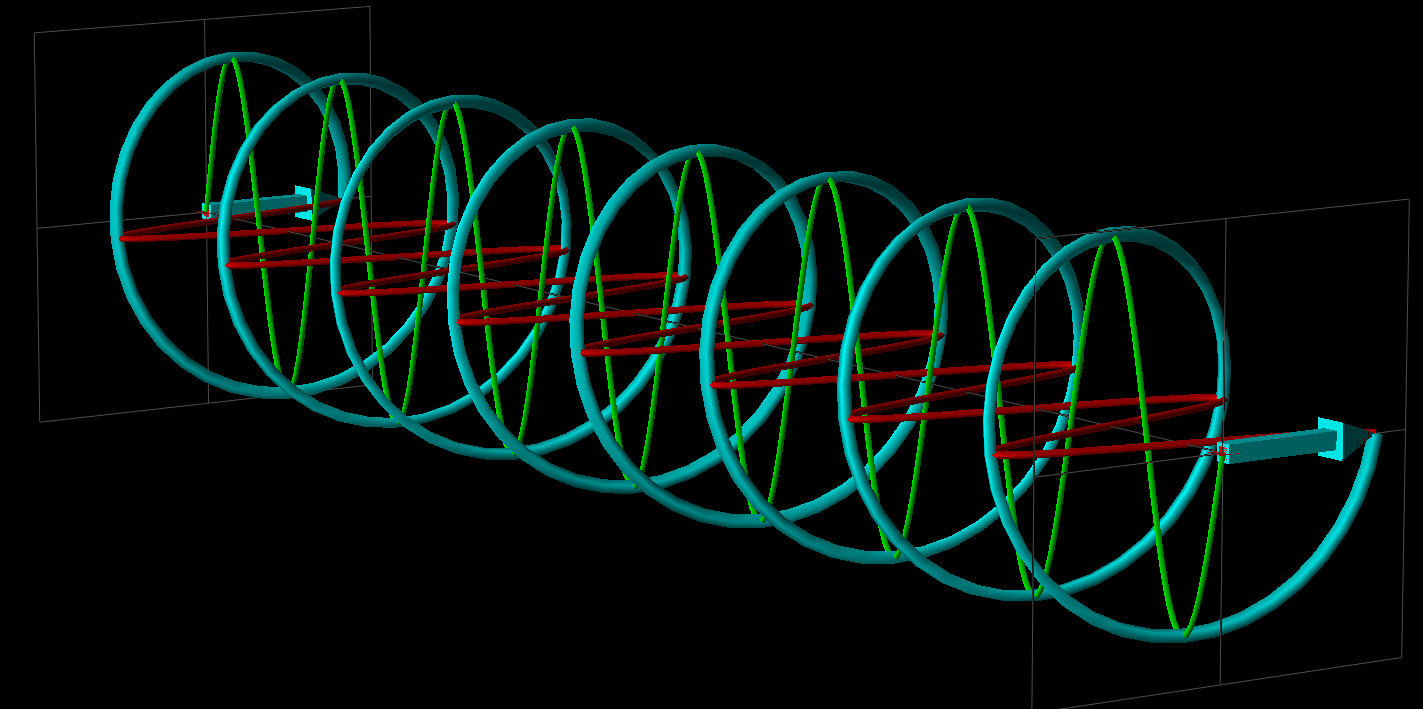
\includegraphics[scale=0.3]{figures/DetailedRightHandPolarization.PNG}
\caption{Circular polarization, where x (red line) and y (green line) component of the electrical field are oscillating forth and back, with equal magnitude to create the circular pattern (blue line)}
\end{figure}

\subsubsection{Elliptical polarization}
For elliptical polarization, the only difference between this type of polarization and circular polarization is the magnitude factor, where the x and y components has different magnitudes. This can be seen on figure 2.28, the magnitude of the y component is greater than the x component, thus resulting in a elliptical pattern.

\begin{figure}[h]
\centering
%\hspace{-1.5cm}
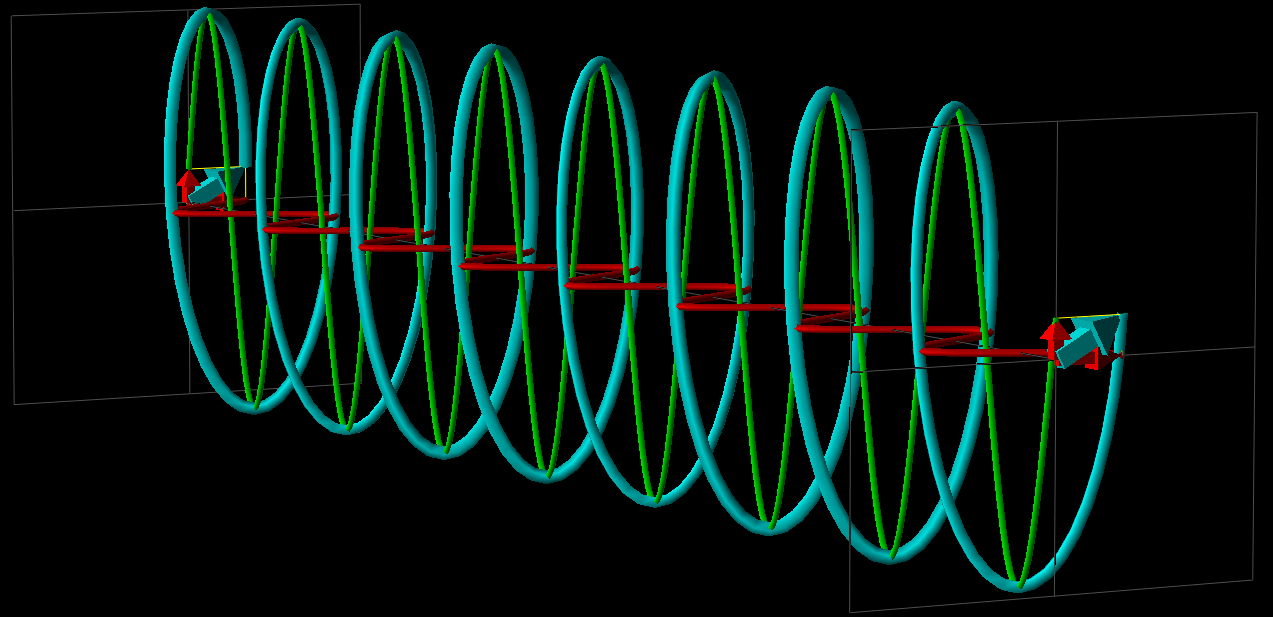
\includegraphics[scale=0.3]{figures/ellipticalPolarization.PNG}
\caption{Elliptical polarization, where x (red line) and y (green line) component of the electrical field are oscillating forth and back, with different magnitudes to create the Elliptical pattern (blue line)}
\end{figure}

\newpage

\subsubsection{Polarization losses}
\begin{figure}[h]
%\centering
\hspace{-2.5cm}
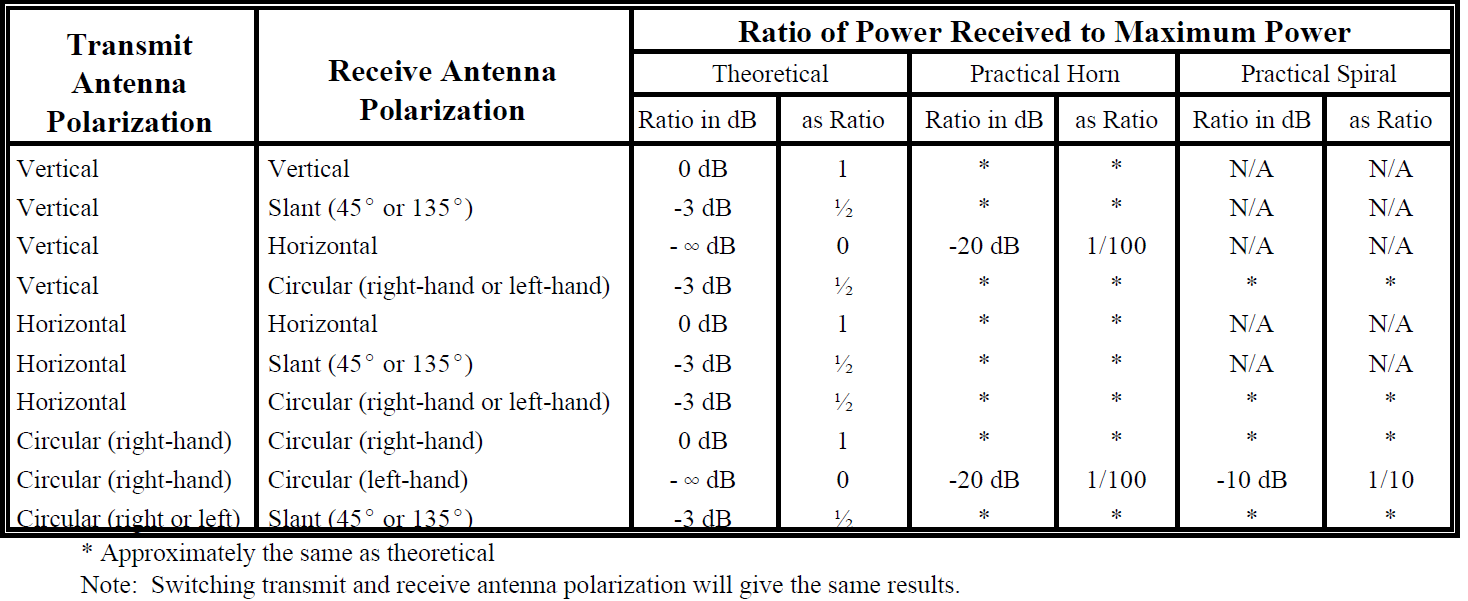
\includegraphics[scale=0.5]{figures/PolarizationLoss.PNG}
\caption{Polarization losses - courtesy of Granite Island Group \cite{gig}}
\end{figure}

Polarization losses occurs when the transmitting and receiving antennas are in a different orientation relative to each other. For a linearly polarized antenna, for example, if the receiving antenna is horizontally polarized and the receiving antenna is vertically polarized, then from the receiving antenna point of view the propagating radio wave will look like a dot in space, which can not be modulated into a meaningful digital signal. If both the transmitter and receiver is right hand circular polarized, then there will be no loss, but if they are opposite of each other, then there will be be huge losses. Another case, is when a linear antenna is transmitting to a circular polarized antenna, this will work but there will be a general loss of 3dB, the good thing about this setup is that the linear antenna can physically rotate without causing huge losses in connection, like the case where both linear antenna is being used on the transmitter and on the receiver. In this thesis, the last case makes the most sense to use, where a linear antenna is mounted on the rocket, and a circular antenna is used on the ground. The reason for this is that most circular polarized antenna are too big to fit inside the rocket, therefore using linear polarized antenna in the rocket is the only option. There will be a general loss of 3dB, but it is better than having two linear polarized antenna, where the consequences are sometimes huge losses, because the rocket can start to rotate and tumble in the air such that the antennas becomes misaligned, Figure 2.29, depicts the losses when using different polarization setup.  

\subsection{Antenna Impedance}
An antenna presents a load impedance or driving point impedance to what whatever system is connected to it terminals. This driving point impedance of an antenna is important in that a good impedance match between the circuit (such as the transceiver) and the antenna is required for maximum power transfer to the antenna. The maximum power transfer occurs when the circuit and antenna impedance are matched. When the antenna and circuit impedance are not matched, the result is reduced antenna efficient because part of the signal is reflected back to the source, due to standing waves along the transmission line, see next section. The reflection coefficient can be determined from the circuit and antenna impedances, and is given by: 

\begin{equation}
   \Gamma = \frac{Z_1-Z_0}{Z_1+Z_0}
\end{equation}

where $Z_1$ and $Z_2$ is the impedances from the circuit and antenna and where $\Gamma$ is a complex number that describes both the magnitude and the phase shift of the reflection. The simplest cases with $\Gamma$ measured at the load are: 

\begin{itemize}
  \item $\Gamma = -1$: complete negative reflection, when the line is short-circuited.
  \item $\Gamma = 0$: no reflection, when the line is perfectly matched.
   \item $\Gamma = 1$: complete positive reflection, when the line is open-circuited.
\end{itemize}

If there is a cable between the antenna and the transceiver, the mismatch creates a voltage standing wave ratio (VSWR) on the cable. The effect of a VSWR on a cable will increase the effect of the cable loss. To compute the VSWR we can use the formula or see this reference \cite{AntennaThoryVSWRCalculator}:

\begin{equation}
   VSWR= \frac{1+|\Gamma|}{1-|\Gamma|}
\end{equation}

Equation (2.75)  is usually given over a bandwidth, so that it is possible to know how much power is reflected by the antenna over a frequency range. To get the return loss $S11$, formula (2.75) can be inverted to: 

\begin{equation}
   |\Gamma|_{s11}= \frac{VSWR-1}{VSWR+1}
\end{equation}

The reflected power back towards the transceiver is given in percentage:

\begin{equation}
   RP = 100|\Gamma|^2
\end{equation}

And in dB:

\begin{equation}
   RP_{dB} = 10log_{10}(|\Gamma|^2) = 20log_{10}(|\Gamma|)
\end{equation}

The amount of power delivered to the antenna is written as $|\tau|$ and is also known as mismatch loss:

\begin{equation}
   DP = |\tau|^2 = 1-|\Gamma|^2
\end{equation}

in dB:

\begin{equation}
   ML_{dB} = 10log_{10}(DP) = 10log_{10}(|\tau|^2) = 20log_{10}(|\tau|)
\end{equation}

So is a VSWR of 3 bad? or how bad is VSWR of 12? There are no specific rules on that, generally the unwritten rule states no higher than a VSWR of 1.7, below is a figure depicting the relationship between VSWR, reflection coefficient $\Gamma$ (s11), total reflected power in percentage and in dB.

\begin{table}[h!]
\centering
\begin{tabular}{|l|l|l|l|}
\hline
VSWR & $\Gamma$(s11) & Reflected Power(\%) & Reflected Power(dB) \\\hline
1.0  & 0.000          & 0.00  & -Infinity     \\ \hline
1.5  & 0.200          & 4.0   & -14.0         \\ \hline
2.0  & 0.333          & 11.1  & -9.55         \\ \hline
2.5  & 0.429          & 18.4  & -7.36         \\ \hline
3.0  & 0.500          & 25.0  & -6.00         \\ \hline
3.5  & 0.556          & 30.9  & -5.10         \\ \hline
4.0  & 0.600          & 36.0  & -4.44         \\ \hline
5.0  & 0.667          & 44.0  & -3.52         \\ \hline
6.0  & 0.714          & 51.0  & -2.92         \\ \hline
7.0  & 0.750          & 56.3  & -2.50         \\ \hline
8.0  & 0.778          & 60.5  & -2.18         \\ \hline
9.0  & 0.800          & 64.0  & -1.94         \\ \hline
10.0 & 0.818          & 66.9  & -1.74         \\ \hline
15.0 & 0.875          & 76.6  & -1.16         \\ \hline
20.0 & 0.905          & 81.9  & -0.87         \\ \hline
50.0 & 0.961          & 92.3  & -0.35         \\ \hline
\end{tabular}
\caption{The relationship between VSWR, $\Gamma$(s11), reflected power in percentage and reflected power in (dB)}
\end{table}
\subsubsection{Vector impedance analyzer (VIA)}
 Unlike an Vector Network Analyzer, which is big and expensive capable of showing more advanced parameters like the VSWR, s11 and a Smith chart (see next section) and transmission losses, a Vector Impedance Analyzer is smaller and cheaper and also capable of showing the VSWR and s11, which are the most important parameters, since everything else, needed in this thesis, can be calculated from these two parameters. Therefore a VIA will be used to characterize the antennas. Below, on figure 2.30, it can be seen the VIA that is used in this thesis.
 
\begin{figure}[h]
\centering
%\hspace{-2.5cm}
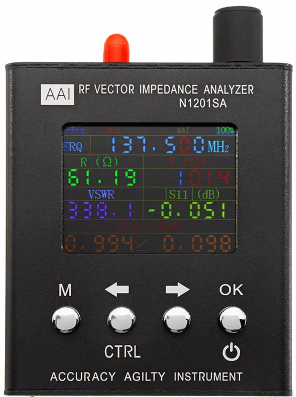
\includegraphics[scale=0.7]{figures/VIA.PNG}
\caption{A vector impedance analyzer (VIA)}
\end{figure}

\subsection{Impedance matching and Smith Chart}
Impedance matching, or Antenna matching is the practice of designing the input impedance of an electrical load or the output impedance of its corresponding signal source to minimize signal reflection from the load. An impedance vector consists of a real part (resistance, R) and an imaginary part (reactance, X), and can be expressed using the rectangular-coordinate form:

\begin{equation}
   Z = R + jX
\end{equation}

The maximum power transferred from the load to the source happens when the load impedance equals to the complex conjugate of the source impedance $Z_l = Z_g^*$, please see this reference\cite{ImpedanceMatching}, which describes why this is the case. In order to accomplish this a matching network is inserted between the load and source:

\begin{figure}[h]
%\centering
\hspace{-1.5cm}
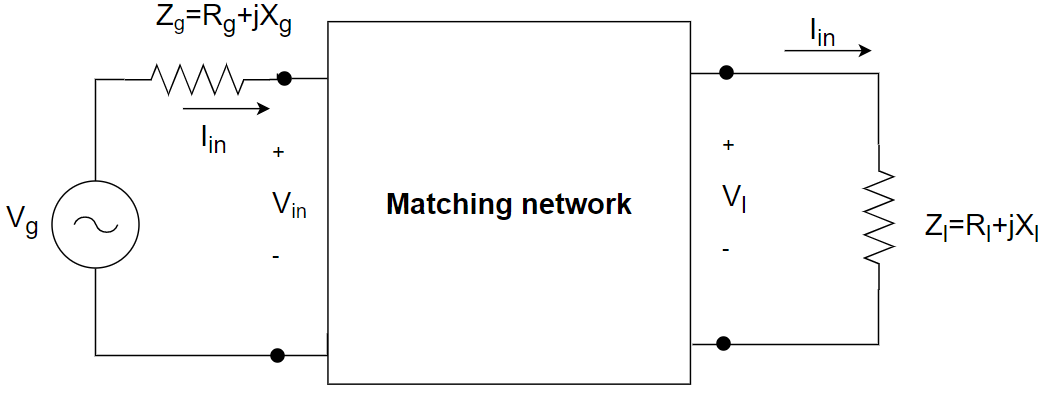
\includegraphics[scale=0.6]{figures/MatchingNetwork.PNG}
\caption{Matching network inserted between the load and source}
\end{figure}

The sole purpose of this matching network is to "transform" the load impedance into an input impedance this \textit{is conjugate matched} to the source, i.e:
\begin{equation}
   Z_{in} = \frac{V_{in}}{I_{in}}=Z_g^*
\end{equation}

For more information about impedance matching, these two references are excellent to read, the first being \textit{Chapter 5 - impedance matching and tuning} by Jim Stiles\cite{ImpedanceMatching1} and the second \textit{Impedance matching} by Iulian Rosu, YO3DAC\cite{ImpedanceMatching2}.

The unwritten rule for most transceivers is that the have a input impedance of 50ohm, based on the theory above, the used antennas also needs to have a impedance of 50ohm, to obtain maximum power transfer from the transceiver to the antennas, and vice versa . In reality this is not the case, for example for a dipole antenna the impedance is $73\Omega$, for a \textit{folded} dipole antenna it is 4 times more than the normal dipole antenna, around $300\Omega$. Depending on what type of load that is used, there are different types of matching networks.The following subsection, describes those that might be used in this thesis, depending on the type of antenna and circuit that is going to be designed.   

In order to impedance match an antenna with a transceiver, or anything else where RF is being transmitted through, a Smith Chart can be used to visualize what type of matching network is needed. Figure 2.32 show a picture of a smith chart, the overall goal is to aim for the center where $Z=1$, in order to do that we can use inductors and capacitors in either a Pi or Tee configuration, to move around the circle and reach the center. 

\begin{figure}[h]
\centering
%\hspace{-2.5cm}
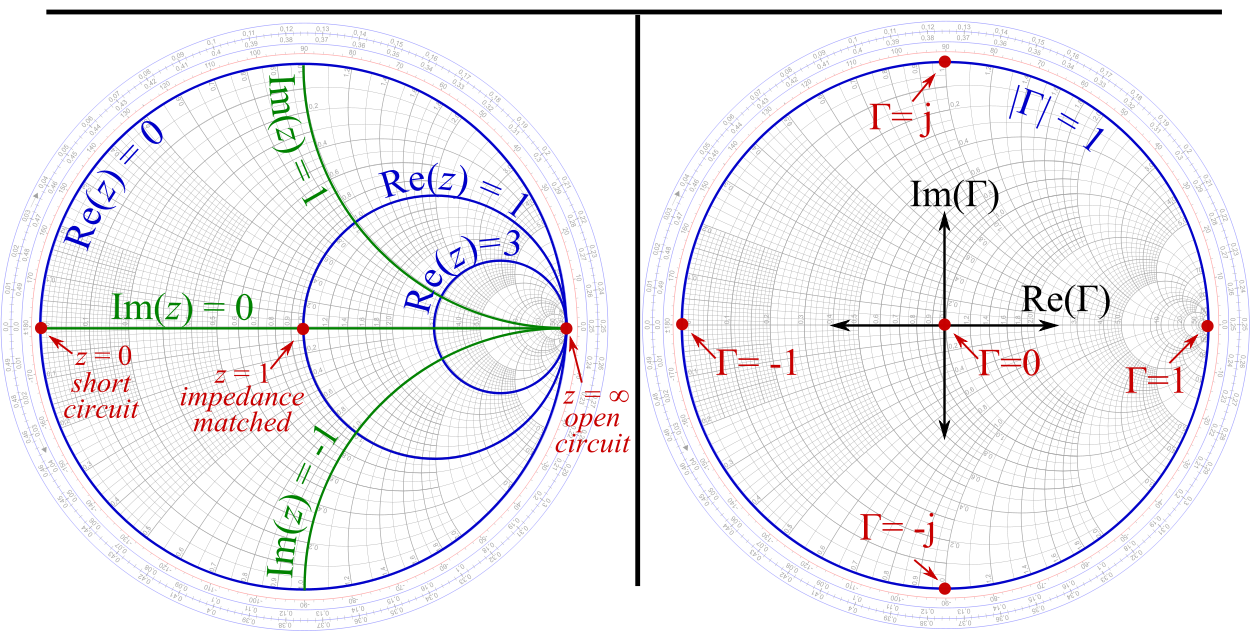
\includegraphics[scale=0.4]{figures/SmithChart.png}
\caption{Smith chart\cite{SmithChart}}
\end{figure}

Figure 2.33 shows the influence a Pi and T network has on the impedance vector A and B. On A it can be seen how the shunt L (inductor) "pushes" A up to the center line, then the series C (capacitor) moves the line down again, and finally the last shunt L, moves the line to the center. For further information on Pi and Tee networks, see section 2.5.8.3 \textit{Tee and Pi networks}.  

\begin{figure}[h]
\centering
%\hspace{-2.5cm}
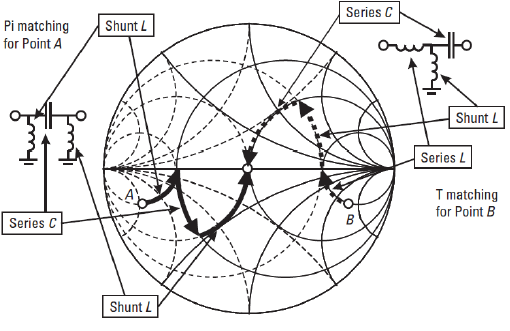
\includegraphics[scale=0.7]{figures/PiTeeSmithChart.PNG}
\caption{Smith chart\cite{SmithChart} with a pi and tee network, showcasing how they influence the impedance}
\end{figure}


\subsubsection{Transmission lines}
The transmission line solution (or a matching stub) is used for rather big antennas, such as dipole, yagi-uda, helical antenna. Basically, a matching stub is a piece of a coaxial cable with appropriated calculation in impedance (Z), overall length etc., which acts as a "Imepdance transformer" between 2 known but unequal impedances $(Z_1,Z_2)$. With the quaterwave formula, it is possible to calculate the intermediate $Z_0$ of a "Quarter Wave" $\frac{\lambda}{4}$ coaxial piece, in order to be able to match 2 different impedances. 

\begin{equation}
   Z_0 = \sqrt{Z_{in}Z_{L}}
\end{equation}

\begin{figure}[h]
\centering
%\hspace{-2.5cm}
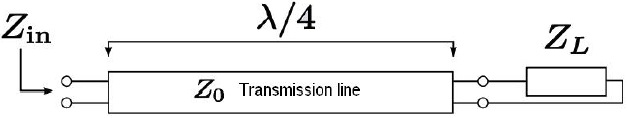
\includegraphics[scale=0.7]{figures/TransmissionLine.PNG}
\caption{Matching stub between to loads}
\end{figure}

The downside of a $\frac{\lambda}{4}$ is that it provides a perfect match at only one frequency. This type of matching network is mostly used for yagi antennas, and cross yagi antennas, see section 2.6.5 \textit{yagi-uda and cross yagi-uda}, but it can also be used for other purposes that needs a coaxial matching, for further information about how to match a yagi and crosyagi antenna, read this reference \cite{YagiMatching}. 

\subsubsection{Microstrip line}
On a RF PCB there will certainly be RF transmission lines (also called microstrip line) going from the antenna connector to the amplifier and from the amplifierr to the tranceiver. This microstrip line has to have an impedance matching the transceiver, of 50ohm. There exits many different microstrip lines, which will not be covered in this thesis, but only the one that is going to be used, which is the simplest version, called \textit{microstrip}. Figure 2.33 show the microstrip line that is used in this thesis, what is important here is that the line must be calculated to have an impedance of 50ohm. The parameters that are important is: Trace thickness T, substrate height H, trace width W and substrate dielectric $\varepsilon_r$ (not seen on the figure). It does not make sense to explain the math behind how to calculate the impedance to be 50ohm, since most online calculators do a great job of that. In this thesis an online calculator will be used for figuring out the exact impedance needed for the microstrip line, see reference for the calculator\cite{MicrostripCalcu}. 

\begin{figure}[h]
\centering
%\hspace{-2.5cm}
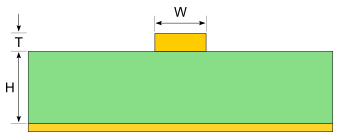
\includegraphics[scale=0.7]{figures/Microstrip.PNG}
\caption{A microstrip line}
\end{figure}

\subsubsection{Tee and Pi networks}
In this thesis a Pi or a Tee network might be used for each transceiver to match the impedance of the antenna with the transceivers. The pi or tee networks consists of inductors and capacitors soldered on the transmission line one the PCB, shorted to ground. Figure 2.34 shows the 4 different typologies, used to match a transmission line, where C is a capacitor and L is an inductor. See also the smith chart in section, 2.5.8 \textit{impedance matching and Smith Chart}.  

\begin{figure}[h]
\centering
%\hspace{-2.5cm}
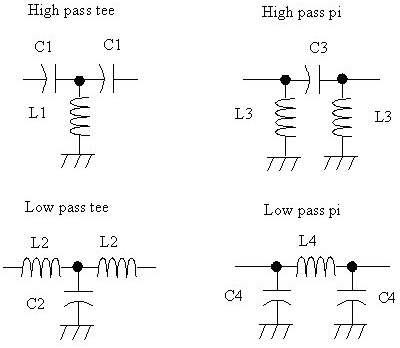
\includegraphics[scale=0.70]{figures/PiTee.PNG}
\caption{Low- and high-pass Pi and Tee networks}
\end{figure}

For further information on how to calculate the parameters of the components and power loss through a Pi/Tee network, it is highly advised to read a text written by a radio amateur, Gary with an amateur licence name of ZL1AN, see reference \cite{PiTeeNetwork}, especially section 1.4 \textit{Pi Matching Networks} and example 1.2, in section 1.4.1.

\section{Different type of Antennas}
There many different types of antennas in the RF world, this thesis will focus only on those antennas that make sense to use for the telemetry system. There are always pros and cons between choosing a given antenna in favour for an other, these pros and cons is defined by different parameters, such as: Antenna radiation pattern, physical look (size and weight), gain, impedance, polarization, beam width and how easy they are to produce and mount either on the rocket or on the ground. The following sub-section will clarify these antennas and their parameters.

\subsection{Half-wave Dipole antenna}
As the name suggest, a center fed half-wave dipole antenna has a total length of $\frac{\lambda}{2}$ where each side elements are $\frac{\lambda}{4}$ long, see figure 2.37. 

\begin{figure}[h]
\centering
%\hspace{-2.5cm}
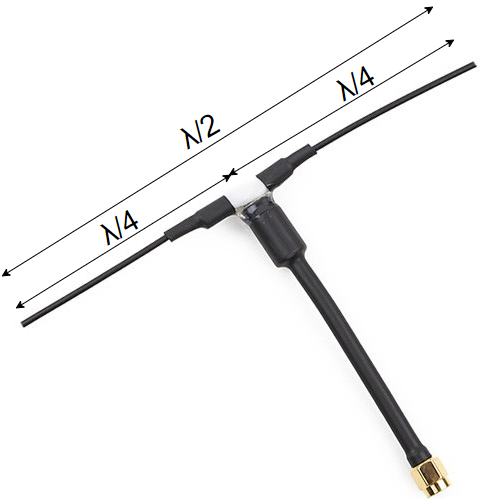
\includegraphics[scale=0.6]{figures/Dipole.PNG}
\caption{Half-wave dipole antenna}
\end{figure}

Since this antenna has been measured many times inside an anechoic chamber, it is therefore used as a reference for other antennas, when it comes to the gain parameter (in dBd = decibel dipole), see section 2.1.3 \textit{What is dB/dBi/dBd/dBW/dBm?}. This antenna is also the building block for many other antennas, such as beam antenna and yagi-uda antennas. In free space - when the antenna is remote from everything else - the theoretical impedance of a physically half-wave long dipole antenna, is $z=73+j42ohm$. The antenna exhibits both resistance and reactance, as can be seen with the imaginary part of the complex number $+j42$, this means that a matching network is needed to decrease the real part of the complex number to 50 ohm, but at the same time removing the imaginary, this is how it is done to achieve the best matching, as stated in section 2.5.8 \textit{impedance matching and smith chart}, especially reference\cite{ImpedanceMatching}. This antenna is linear polarized, it has a gain of 2.15 dBi and a radiation pattern that can be observed on figure 2.20 and 2.21 (further up). From figure 2.21b it can bee observed that the Half-power beam width is around 80 degrees. 

\subsection{Sleeved Dipole antenna}
A sleeved dipole, is like half-wave dipole, but made in such a way that one of the $\frac{\lambda}{4}$ elements are "cased" on top of the coax cable, while the other side is exposed, as see on figure 2.38a and 2.38b, both sides a equally long, but the radius of the aluminum casing is larger than the radius of the exposed coaxial cable, by changing he radius of the aluminum casing one can achieve an impedance of 50ohm at a given operating frequency. The center feed point is in the middle, between the metal casing(aluminum) and the exposed coaxial core (white). The pros of this antenna compared to the half-wave dipole antenna, is the way it is constructed, this allows for easier mounting on the rockets hull and that the antenna is already matched to 50ohm. The downside of this antenna, the radiation pattern is probably the same as a half-wave dipole, since the thickness of the aluminum casing will effect how the radiation pattern looks like. Other than the impedance, the rest of the parameters should be fairly the same as a half-wave dipole antenna. 

\begin{figure}[h!]
  \centering
  \begin{subfigure}[b]{0.65\linewidth}
    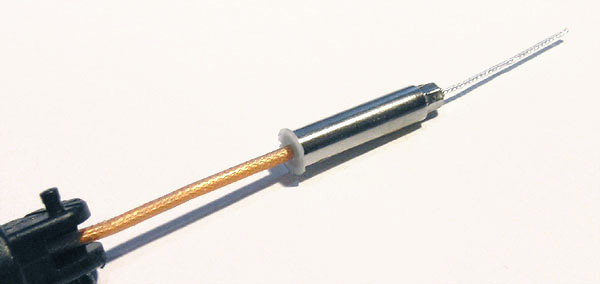
\includegraphics[width=\linewidth]{figures/SleeveDipole.jpg}   
    \caption{Sleeved dipole}
    \end{subfigure}
  \begin{subfigure}[b]{0.65\linewidth}
    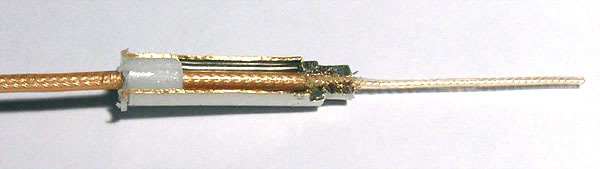
\includegraphics[width=\linewidth]{figures/SleeveDipoleOpen.jpg}
    \caption{Sleeved dipole open}
  \end{subfigure}
  \caption{A Sleeved dipole antenna, usually bought from china}
\end{figure}

\subsection{Folded dipole antenna}
A folded dipole is usually used as the driven element on a yagi-uda antenna, the reason for using a folded dipole and not just a normal half-wave dipole, has to do with the impedance. The folded dipole, has a impedance of around $300\Omega$, this can be used in a positive way, since the parasitic (directors) elements on a yagi-uda antenna, see section 2.6.8 \textit{Yagi-uda and cross yagi-uda}, decreases the impedance, meaning if one choose to use a normal half-wave dipole, depending on amount of directors, the impedance of the yagi-uda antenna will probably fall below $50\Omega$, thus using a folded dipole, increases the impedance, and allows for more directors to be used to increase the directivity of a yagi-uda antenna. Furthermore, the folded dipole has a wider bandwidth than a normal half-wave dipole. Figure 2.39 shows an example of a folded dipole, beside this the rest of the parameters is quite the same as a dipole antenna. 

\begin{figure}[h]
\centering
%\hspace{-2.5cm}
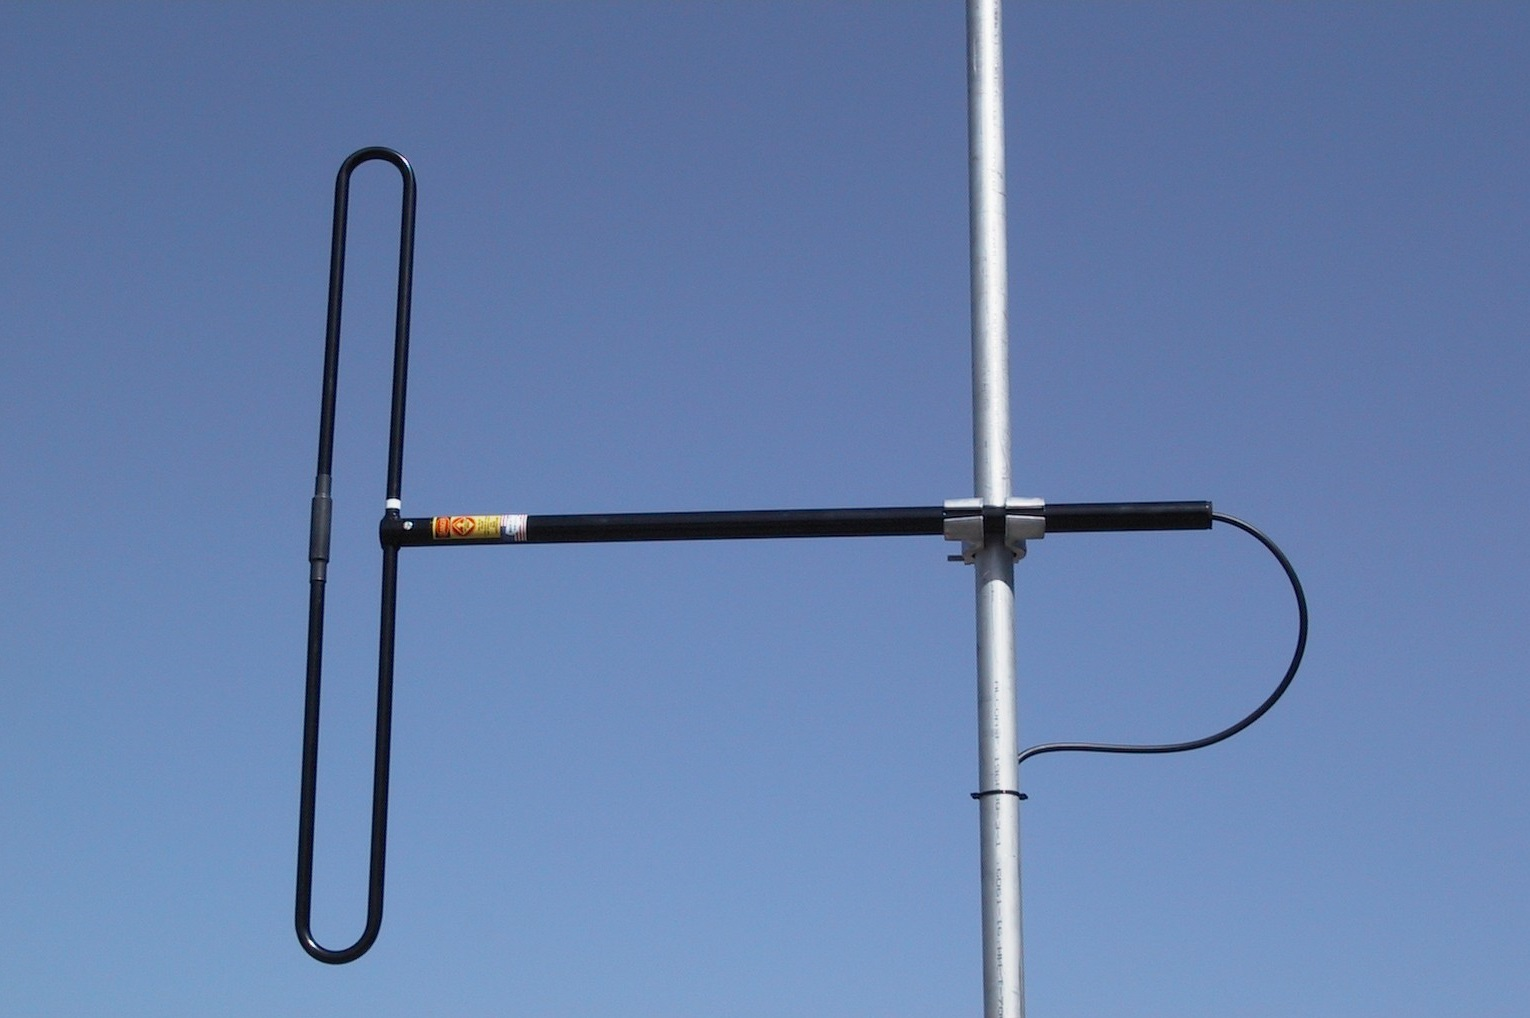
\includegraphics[scale=0.9]{figures/FoldedDipole.jpg}
\caption{Folded Dipole}
\end{figure}

\subsection{Quaterwave monopol antenna}
A quaterwave monopol antenna has a length of $\frac{\lambda}{4}$, and usually is above some kind of a ground plane, either the earth itself or a metal ground plane, with the same radius as the chosen wavelength. This antenna is also linear polarized, and as the name states, the monopol antenna only have one "pole" compared to a dipole, which has both elements sticking from the center. A monopol antenna is fed at the end of the wire (closest to ground), but the ground plane acts as a reflector/mirror, thus allowing it to behave as a dipole antenna, but less effective. Because of this, the radiation pattern only exits above the ground, meaning only half of the dipole. Figure 2.40, show the gain for a quaterwave monopol antenna, but also the radiation pattern, as described above it is only half of the sphere, therefore the energy is directed to the other half meaning the gain of a quaterwave monopol antenna is $G=2.15+3dB=5.15$ for a perfect ground plane, but in reality such a ground plane does not exits, thus the gain is usually closer to a dipole antenna. The impedance of this type of antenna in free space is around $Z=36.5+j21.25$\cite{ImpedanceMonopol}, this is close to $50\Omega$ one way to solve this problem is to build a ground plane for the antenna, made out of 4 to 5 radials, acting as ground plane, then bend them approximately 35-45 degrees downwards to increase the impedance to $50\Omega$, see figure 2.41. 

\begin{figure}[h]
\centering
%\hspace{-2.5cm}
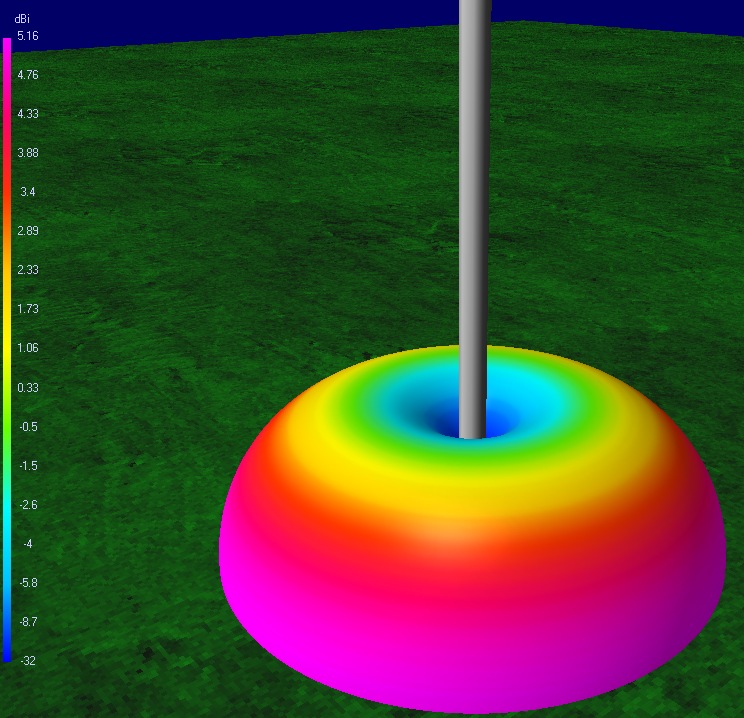
\includegraphics[scale=0.50]{figures/quaterwaveMonoplAntenna.PNG}
\caption{Gain and radiation pattern for a quaterwave monopol antenna}
\end{figure}

\begin{figure}[h]
%\centering
\hspace{-1cm}
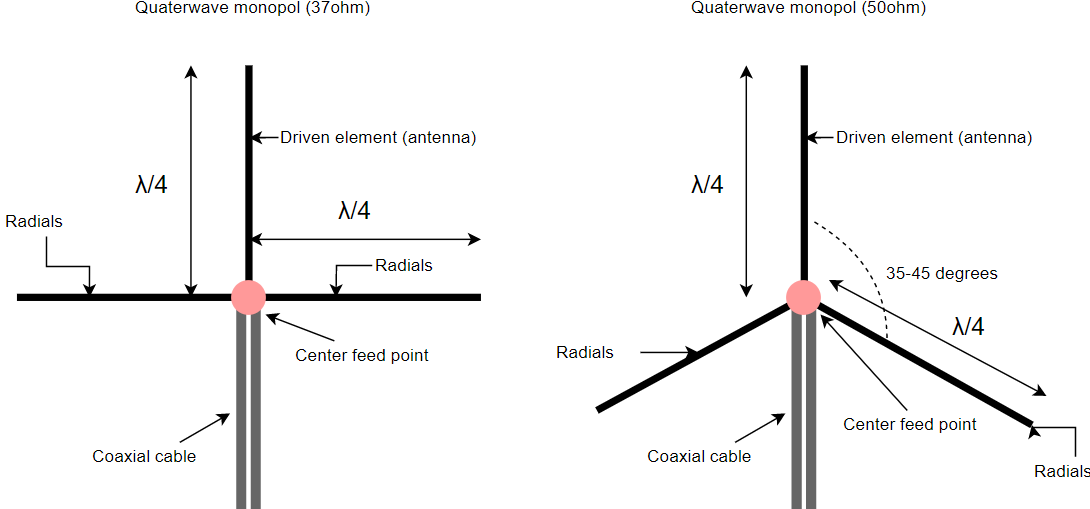
\includegraphics[scale=0.55]{figures/QuaterWaveMonopolAntennaRadials.PNG}
\caption{a 2-dimensional visualization of two quaterwave monopol antenna with radials perpendicular to the antenna and radials bent 35-45 degrees}
\end{figure}

\subsection{Helical antenna}
A typical helical antenna consists of a single conductor wound into a coil that is attached to a pipe made of a non-conducting material, such as plastic. The pipe is attached to a conducting ground plane, made of aluminum or copper. The coil goes trough the ground plane, without touching it, and is soldered to a SMA connector, where the antenna is fed. See figure 2.42. 

\begin{figure}[h]
\centering
%\hspace{-1cm}
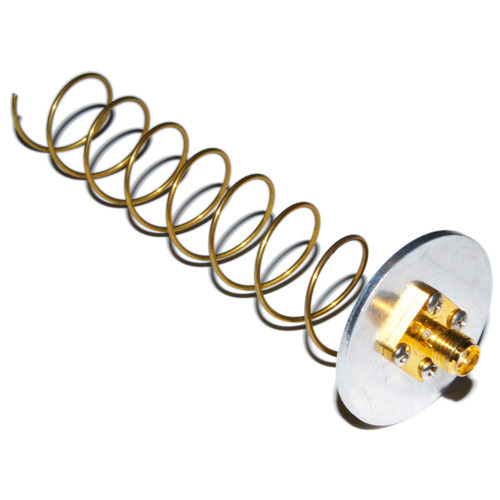
\includegraphics[scale=0.6]{figures/HelixAntenna.jpg}
\caption{A simple helical antenna\cite{HelicalAntenna}}
\end{figure}

A helical antenna can operate in 3 different modes: normal mode, axial mode and conical mode. The first mode make the antenna radiate like dipole antenna, where the radiation pattern is onidirectional. The axial mode, makes the antenna directional like a yagi-uda or any other high gain antenna, it is also the only shape where it is circular polarized (RHCP or LHCP depending on which direction the coil is wraped). The conical mode makes the antenna radiate in a v-shape. See figure 2.43. 

\begin{figure}[h]
\centering
%\hspace{-1cm}
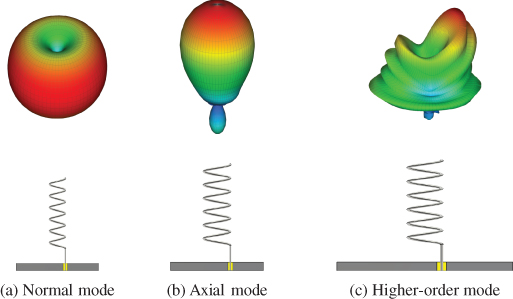
\includegraphics[scale=1.3]{figures/HelicalMode.png}
\caption{helical antenna modes\cite{HelicalMode}}
\end{figure}

For any of the specific modes, there are common parameters used to define the what mode a helical antenna is in. These parameters are also used when simulating and constructing the antenna. See references, \cite{ARRL} page 19-7 to 19-8, \cite{HelicalModeMath} slide 2 and 3, for information about where the below parameters comes from:

\begin{itemize}
  \item $\lambda$ is the wavelength, in meters.    
  \item $D$ is the diameter of the helix, in meters.
  \item $d$ wire diameter, in meters.
  \item $C$ is the circumference of the helix, which equals to $\pi D$, in meters.
  \item $N$ is the number of turns.
  \item $\alpha$ is the pitch angle, given by $\tan^{-1}\Big(\frac{S}{\pi D}\Big)=\tan^{-1}\Big(\frac{S}{C}\Big)$, in degrees.
  \item $S$ is the gap spacing in-between turns, which equals to $C \tan(a)$, in meters.
  \item $L$ is length of one turn, given by $\sqrt{S^2+C^2}$, in meters.
  \item $A$ is axial length, given by $NS$, in meters.
  \item $NL$ is total length of wire, in meters.
  \item $R$ is the diameter of the ground plane, given as .
  \item $S_g$ is spacing form ground plate to the beginning of the helix's first turn, in meters.
\end{itemize}

It is easier to visualize some of the parameter on figure 2.44.

\begin{figure}[h]
\centering
%\hspace{-1cm}
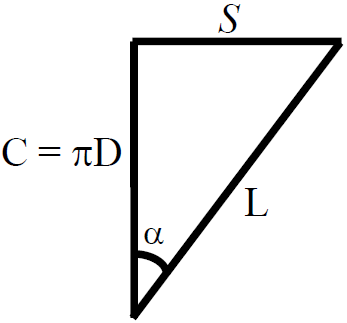
\includegraphics[scale=0.5]{figures/TriangleMath.PNG}
\caption{Simplification of the parameters of a helical antenna}
\end{figure}

On the ground a directive circular polarized antenna is need to track the rocket, therefore the best helical mode is the axial mode. For this thesis only the theory behind the axial mode will be shown. In order to make a helical antenna radiate in the axial mode the following condition must be met:

\begin{table}[h!]
\centering
\begin{tabular}{|l|l|}
\hline
Parameter                          & Range                                                   \\ \hline
Cirumference (meters)              & $\frac{3}{4}\lambda \leq C \geq \frac{4}{3}\lambda$     \\ \hline
Pitch Angle (degrees)              & $\ang{12} < \alpha < 16 $                               \\ \hline
Number of Turns (unitless)         & $N > 3$                                                 \\ \hline
Wire Diameter (meters)             & $.005 < \frac{d}{\lambda} < 0.05$                        \\ \hline
Ground Plane Diameter (meters)     & $0.8\lambda \leq R \geq 1.1\lambda$                     \\ \hline
Spacing to the first turn (meters) & $S_g \approx .12\lambda$                                \\ \hline
\end{tabular}
\caption{Condition that must be met in order to have helical antenna radiating in axial mode}
\end{table}

The impedance of a helical antenna in axial mode is: 

\begin{equation}
   Z_0 = 140\frac{C}{\lambda}
\end{equation}

To calculate the gain of a helical antenna, two equation can be used, one is from the ARRL book\cite{ARRL} page 19-8 and the other is from Wikipedia\cite{HelicalAntennaWiki}, the result of these two formulas is close to each other, but both with be used, for reference sake.  

\begin{equation}
   GARRL_{dBi} = 11.8+10log_{10}\Big(\Big(\frac{C}{\lambda}\Big)^2\Big(\frac{NS}{\lambda}\Big)\Big)
\end{equation}

\begin{equation}
   GWIKI_{dBi} = 10log_{10}\Big(15\Big(\frac{C}{\lambda}\Big)^2\Big(\frac{NS}{\lambda}\Big)\Big)
\end{equation}

The beam-width of the helical antenna (in degrees) at half-power points, see section 2.5.4 \textit{Radiation pattern}, is given by (\cite{ARRL} page 19-8):

\begin{equation}
   HPBW \approx \frac{52}{\frac{C}{\lambda}\sqrt{\frac{NS}{\lambda}}}
\end{equation}

As it can be seen above the half-power beam width, is mostly depended on the number of coil turns N.
The impedance of a helical antenna in axial mode, is around 110 to 130Ohm, this is too high for matching with a transceiver, therefore a matching network is needed to combat this problem. There are many different type of matching networks for a helical antenna. They all have their pros and cons, some of them are easy to build and implement, while others are harder to build, but does not distorted the bandwidth of the antenna. In this thesis, the easiest matching network to build and implement will be chosen, since the narrow bandwidth is not a problem for the use case in this thesis. On the internet their exists a forum where helical antennas are being discussed, a solution to how to build and tune a helical is proposed, It is highly recommend to check out the reference \cite{RCGroups}, see thread \#7, for the type of possible matching networks. For this thesis the first \textit{The Hecker transformer} has been chosen, since it is the easiest to build and implement. It is basically a triangle made out of a conducting metal, aluminum or copper, that is soldered to the coil and wraps around for a approximately a half turn. This metal piece can reduce the impedance closer to the desired 50Ohm, see figure 2.45.  

\begin{figure}[h]
\centering
%\hspace{-1cm}
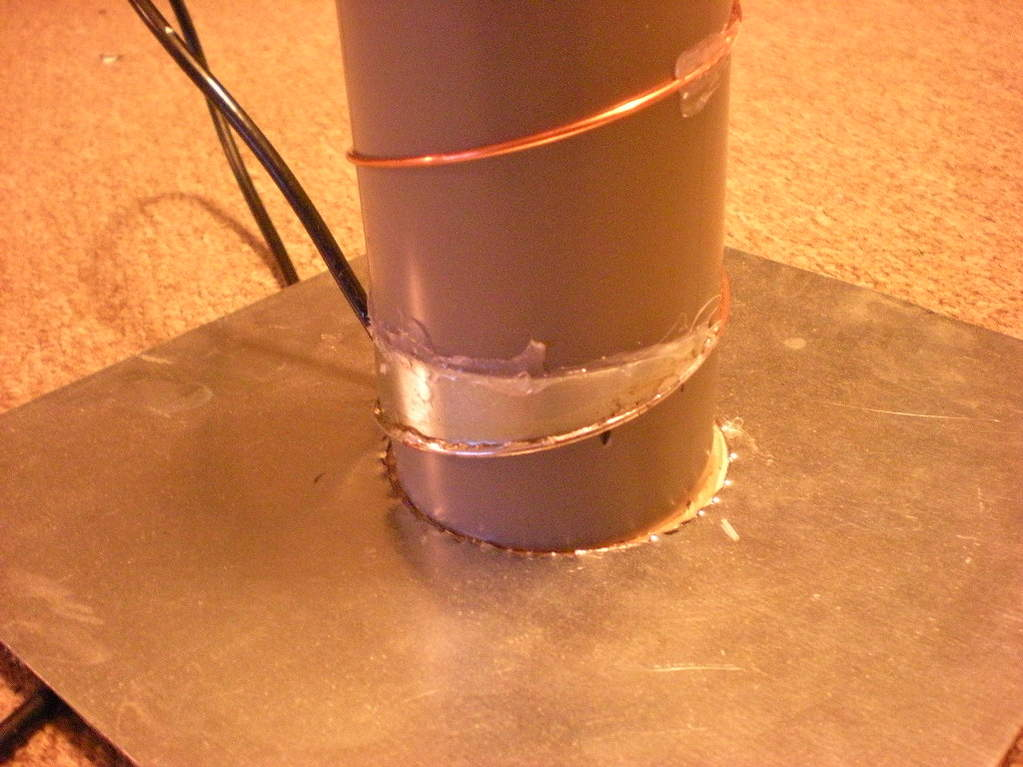
\includegraphics[scale=0.8]{figures/FormerHelical.jpg}
\caption{The Hecker transformer used to lower the impedance of a helical antenna}
\end{figure}

\subsection{Microstrip Patch antenna}
A microstrip antenna, or commonly referred to as \textbf{patch antenna}, is an antenna printed on a circuit board. This type of antenna is relatively small (depending on the frequency) and is so versatile that it is hard to state exactly what the parameters are of a general patch antenna. For the most part, they are directive, either linear or circular polarized, thin and weighing close to nothing. It is out of the scope of the this thesis to explain the theory behind how to produce one of these, therefore It is much easier to buy a standard patch antenna operating at 2.4-2.5Ghz (same frequency as the transceiver) and then test them. The pros of this antenna, is that it can be fitted inside the rocket, without the need of having something sticking out from the rocket. Because it is directive the gain will certainly better than a dipole or quaterwave monopol antenna. The cons are that the field-of-view is narrower for this type of antenna (because of higher gain) means that the antenna needs to be mounted in a special way such that it is aiming correctly towards the ground.  

\begin{figure}[h]
\centering
%\hspace{-1cm}
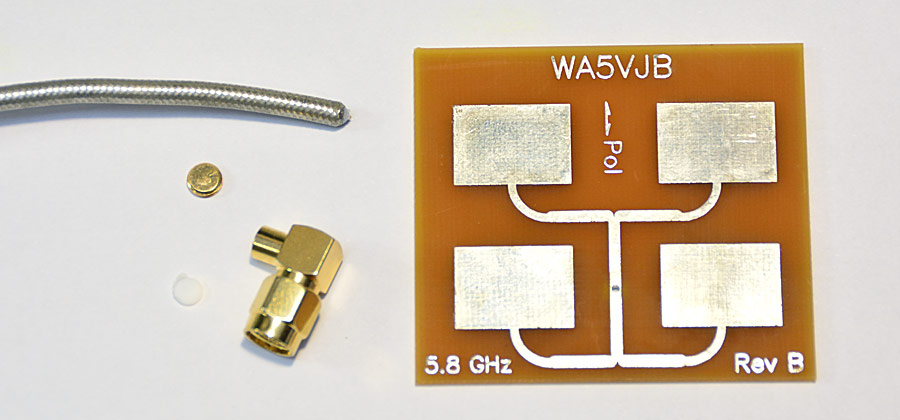
\includegraphics[scale=0.5]{figures/PatchAntenna.jpg}
\caption{Patch antenna, in this case it is an array patch antenna, since there are 4 of the driven elements\cite{PatchAntenna}}
\end{figure}

\subsection{Yagi-uda and cross-yagi-uda antennas}
The Yagi-uda antenna is one of the most brilliant antennas designed, it can be seen on nearly every rooftops, pointing towards the RF source. A yagi-uda antenna is a high gain antenna operating in the HF to UHF bands about 3Mhz to 3Ghz, and is linear polarized. The antenna consists of 5 basic parts: a reflector, a driven element usually it is a folded dipole, multiple directors to direct he RF wave straight forward, a center rod for all the elements to be attached to and finally a matching network for the driven element.

The Reflector reflects the RF wave back to the dipole, to decrease backwards side lobes and increase the gain of the forward beam. The driven element can either be a dipole or a folded dipole, remember in section, 2.6.3 \textit{Folded dipole antenna}, it is explained that the impedance of a yagi-uda is dependent on how many directors is used, since increasing the amount of directors will the gain but also decrease the impedance. If a normal dipole with the impedance of $73\Omega$ is used then only a few directors can be added before the impedance is reduced to $50\Omega$, thus the antenna will not be as directive as theoretically possible. That is why a folded dipole is used, since it has a impedance of around $300\Omega$ many more directors can then be added before reaching $50\Omega$, thus further increasing the gain. The directors, will focus the RF wave in one direction to increase the gain, they are not connected to the driven element in way (folded dipole), only mounted on the center pole. The directors are also called parasitic elements, since they influence the dipole radiation pattern, see section 2.5.5.4 \textit{Reative near-field region}. Even though one can use the directors to lower the impedance to $50\Omega$, one may not want to do this, since the drawbacks will be a very narrow field-of-view, meaning one has to point very precise in order to avoid antenna misalignment, As explained in section 2.4.1 \textit{Antenna misalignment attenuation} and 2.5.2 \textit{Directivity, efficiency and gain}. To avoid this problem a matching stub can be used, which is explained in section 2.5.8.1 \textit{Transmission lines}, on how to add a matching stub to a yagi-uda antenna, please read this reference \cite{YagiMatching}. For this thesis the yagi-uda antenna will not be build but bought and used as a reference to the helical antenna, they are inexpensive to buy and work brilliantly out of the box.  

\begin{figure}[h]
\centering
%\hspace{-1cm}
\includegraphics[scale=0.5]{figures/yagi-uda.png}
\caption{A yagi-uda antenna, with 1 reflector, 1 driven element a folded dipole and multiple directors\cite{YagiUda}}
\end{figure}

Another type of a yagi-uda antenna is the cross-yagi-uda antenna. This antenna consists of two similar yagi-uda antenna, attached perpendicular to each other. A cross-yagi-uda antenna is a high gain circular polarized antenna, just like the helical antenna. The circular polarization can be achieved in two ways, either by creating a phasing stub (made out of coaxial cable), to delay one of the yagi antenna by 90 degrees to induce a rotation in the RF field or the rotation can be induced simply by shifting one of the yagi antenna by distance of $\frac{\lambda}{4}$, see figure 2.48 and 2.49. The pros of this type of antenna, is that once it is build and with a clever matching setup, it can be used in linear polarized mode (either vertically or horizontally), or in circular polarized mode, by merging both antenna together. The cons of both yagi-uda an especially cross-yagi-uda is the complexity of constructing one, compared to constructing a helical antenna. 

\begin{figure}[h]
\centering
%\hspace{-1cm}
\includegraphics[scale=0.8]{figures/PhaseStub.PNG}
\caption{Phase stub solution for circular polarization\cite{YagiMatching}}
\end{figure}

\begin{figure}[h]
\centering
%\hspace{-1cm}
\includegraphics[scale=0.8]{figures/CrossYagi.PNG}
\caption{Cross-yagi-uda antenna with a physical solution to induce circular polarization\cite{YagiMatching}}
\end{figure}

\newpage

\section{Detailed Link Budget}
The link budget is a compilation of all the gains and losses in a radio communication system. By assuming the transmit power is in dBm with all the relevant gains and losses in dB and subtracting the required received signal (RSL, in dBm), the link margin is obtained. The link margin provides a measure of robustness for radio link. The beauty of a link margin is that, the better one understands the gains and losses in the link budget, by simulating and modeling the circumstances, the smaller the link margin can be and still achieve a robust radio connection. An experienced RF designer will be able to come up with a very precise link budget and a good estimate of what the link margin should be, mainly based on experience. What makes it so hard is that some of the losses in a link budget are based on availability requirements, and therefore the actual losses are not always present. Availability requirements, are losses that might or might not exists on the day of testing, such as rain, clouds, multipath losses and Fresnel zone. They all depends on the day, where the test setup set placed and how the environment is between the transmitter and receiver. For example, a link budget has been made for a given scenario that scenario changes because of unexpected reasons, this could be that the military changes their minds on where the ground mission control should be stationed to track the rocket, thus the tracking system has to be moved a significant distance, to a terrain with unfavorable conditions. This example, is an argument for having a conservative link margin, but what should this margin be? 6, 10, 15 or even higher? The author of this thesis has asked experienced RF designers and members of \textit{Copenhagen Suborbitals}\cite{CopenhagenSuborbitals} (a non-profit amateur rocket club), where the conclusion was that the margin should be no lower than 15 dB, for this case scenario. Any lower than \textit{15dB} a robust connection at distance of 9km cannot be guaranteed, but it will still be possible to receive data.

The link budget consist of 4 subcategories, these are: transmitter side, channel losses, other losses and receiver side. Figure 2.50 shows an overview a link budget, with all the losses and gains, it can also be observed that there are keyword, such as EIRP, RSL and RSSI, these will be clarified in the following subsections: 

\begin{figure}[h]
\centering
\hspace*{-2.3cm}
\includegraphics[scale=0.70]{figures/LinkBudgetOverview.PNG}
\caption{Overview of a link budget}
\end{figure}

\subsection{Transmitter side}
The transmitter side usually consists of 4 physical parts, the PCB (the source of the RF signal), SMA connectors, coaxial cable and finally the antenna. The total sum of all the losses and gains from these 4 physical part, will result in the Effective Isotropic Radiated Power (EIRP), in detail the formula is:

\begin{equation}
   P_{EIRP} = P_t+L_{balun}+P_{PAE}+L_{filter}+L_{match}+L_{con}+L_{cab}+G_{t} \quad [dB]
\end{equation}

where:

\begin{itemize}
    \item $P_t$ is the gain from the transceiver output power.
    \item $L_{balun}$ is the insertion loss of the balun, between the transceiver and power amplifier.
    \item $P_{PAE}$ is the gain from the external power amplifier.
    \item $L_{filter}$ is the insertion loss of the band filter.
    \item $L{match}$ is the matching loss between the antenna and the transceiver (PCB).
    \item $L_{con}$ is the losses from SMA connectors (Tx side).
    \item $L_{cab}$ is the loss due to the length of the coaxial cable (Tx side).
    \item $G_{t}$ is the gain from the antenna.
\end{itemize}

From $P_t$ to $L_{filter}$ is actually the PCB that generates the RF source. Beside the losses from the balun and band filter, other losses can be occur, due to bad PCB design, these type of losses is hard to estimate, in this thesis they will be neglected.

\subsection{Channel losses}
The channel loss is the hardest gain/loss to estimate, since it includes so many parameters that individually are hard to estimate, but mixed together even harder to estimate, they are all described from section 2.3.1 to 2.3.3, the formula is 

\begin{equation}
   L_{Chan} = L_{fs}+L_{prop}+L_{mp} \quad [dB]
\end{equation}

Where:

\begin{itemize}
    \item $L_{fs}$ is the loss from Free-space attenuation.
    \item $L_{prop}$ is the propagation losses from: rain, clouds and atmospheric attenuation.
    \item $L_{mp}$ is the losses from multipath attenuation, Fresnel zone, diffraction, doppler spread.
\end{itemize}

It is very important to note that the Free-space attenuation $L_{fs}$ might be replaced with the Two-ray ground bounce multipath $L_{gbm}$, as stated in in section 2.3.2.1 \textit{Two-ray ground bounce multipath} see last paragraph about the \textit{crossover point}. If this is the case the formula will look like this:

\begin{equation}
   L_{Chan} = L_{gbm}+L_{prop}+L_{mp} \quad [dB]
\end{equation}

\subsection{Other losses}
Other losses is basically the thesis specific losses, explained in section 2.4 \textit{Thesis specific losses}, but it could be other losses that have not been covered in this thesis.

\begin{equation}
   L_{Other} = L_{ama}+L_{pol}+L_{rocket} \quad [dB]
\end{equation}

\begin{itemize}
    \item $L_{ama}$ is the loss from antenna misalignment, between the transmitter and receiver.
    \item $L_{pol}$ is polarization mismatch losses.
    \item $L_{rocket}$ is the loss occurring when the rocket itself blocks the transmitted RF signal. 
\end{itemize}

\subsection{Receiver side}
For the receiver side, there are two keywords Received Signal Level (RSL) and Received Signal Strength Identification (RSSI) to explain, see figure 2.52. In this thesis the RSL is defined as: 

\begin{equation}
   P_{RSL} = P_{EIRP}+L_{Chan}+L_{Other}+G_{r}+L_{cab}+L_{con}+L_{match} \quad [dB]
\end{equation}

where:

\begin{itemize}
    \item $P_{EIRP}$ is described above.
    \item $L_{Chan}$ is described above.
    \item $G_{r}$ is the gain from the receiver antenna.
    \item $L_{cab}$ is the loss due to the length of the coaxial cable (Rx side).
    \item $L_{con}$ is the losses from SMA connectors (Rx side).
    \item $L_{match}$ is the matching loss between the antenna and the transceiver (PCB).
\end{itemize}

In this thesis RSSI is defined as: 

\begin{equation}
   P_{RSSI} = P_{RSL}+L_{filter}+P_{LNAE}+L_{balun} \quad [dB]
\end{equation}

where:

\begin{itemize}
    \item $P_{RSL}$ is described above.
    \item $L_{filter}$ is the insertion loss of the band filter.
    \item $L_{LNAE}$ is the gain from the external Low noise amplifier.
    \item $L_{balun}$ is the insertion loss of the balun, between the transceiver and power amplifier.
\end{itemize}

Some transceiver (not the one used in this thesis) has an internal RSSi measurement unit, which either can be before the transceiver's internal LNA or after. If the RSSI unit is before the internal LNA, then the internal LNA needs to be added to the formula (2.93), unless the datasheet states that the LNA is a part of the RSSI value. 

The link margin is defined by 

\begin{equation}
   LM = P_{RSSI}+P_{RS} \quad [dB]
\end{equation}

where:

\begin{itemize}
    \item $L_{RSSI}$ is described above.
    \item $P_{RS}$ is the gain form the transceiver sensitivity, can be acquired from the datasheet.
\end{itemize}

\section{RF PCB design rules}
To fully explain the theory behind designing a RF Printed Circuit Board (PCB), will be out of the scope of this thesis. What makes sense, is to shortly look at the design rules that helps reduces any losses from the PCB itself. A good PCB design is equally important as a good link budget.  

The first version of the PCB designed for this thesis, is a 4 layer PCB. The 4 layer setup allows for more possibilities than a standard 2 layer board, see figure 2.53. The layers are in the following order: copper 1 (1oz), dielectric layer (4.29), copper 2 (1oz), dielectric layer (3.96), copper 3 (1oz), dielectric layer (4.29), copper 4 (1oz). The 4 layer design, allows for wires to be routed in the middle layers, reducing design complexity, furthermore, the 4 layer design has a dialectic material that is thinner and with a constant that is lower than for a 2 layer design, this means the wire thickens for microstrip impedance matching decreases significantly. See the figure B.1 and B.2 in appendix B, they show the huge difference in the width required for a transmission line, for a 4 layer vs 2 layer PCB's.   

\begin{figure}[h]
\centering
%\hspace*{-2.3cm}
\includegraphics[scale=0.8]{figures/PCB4.PNG}
\caption{4 layer pcb from PCBWay \cite{PCB}}
\end{figure}

Beside the above positive thing about a 4 layer PCB for RF design, there are some general rules to follow when designing a RF PCB board. Figure C.1 on appendix C, is a very good rule of thumb to follow.   


%probably not important, since a prototype is enough for this bachelor, so write only about the schematics compared to insertion loss for the link budget.

\section{Framing and Modulation (MultiCeiver\texttrademark and Shockburst\texttrademark)}
%% DU HAR 2 timer!


